\documentclass[11pt]{ctexart}
\usepackage[margin=2.4cm]{geometry}
\usepackage{amsmath,amssymb}
\usepackage[super,square,numbers]{natbib}
\usepackage{booktabs}
\usepackage{graphicx}
\usepackage{multirow}
\usepackage{tikz}
\usetikzlibrary{arrows.meta,positioning,shapes.geometric,calc}
\usepackage{caption}
\usepackage[hidelinks]{hyperref}
\usepackage{xcolor}

\captionsetup{font=small,labelfont=bf}
\newcommand{\fcntm}{FC-NTM}

\title{\bfseries 面向双字段短文本的字段协同神经主题模型\\[4pt]
       \large ——缺失字段推断、字段视角读出与冗余度度量的实证研究}
\author{王洪利\\[2pt]{\small 哈尔滨工业大学土木工程学院}\\[1pt]{\small 2010254508@qq.com}\\[8pt]
        满庆鹏\textsuperscript{*}（通讯作者）\\[2pt]{\small 哈尔滨工业大学土木工程学院}\\[1pt]{\small manqp@126.com}}
\date{\today}

\begin{document}
\maketitle

\begin{abstract}
真实文本常由功能分工的两个字段构成（如标题与正文），而把整条记录拼接成无结构词袋会丢弃
字段分工。本文提出字段协同神经主题模型 \fcntm{}：为两个字段分别建立条件变分流，两条流共享
同一线性主题解码器，以跨字段重构与字段一致性正则把字段关系编码进共享主题空间，并以字段级
词掩码与背景字段整体置零处理部分观测与整体缺失；同一训练结果支持解码器 $\beta$ 读出与
类 TF-IDF 读出两种主题词读出。

本文的应用背景是工程文献的主题结构挖掘：土木工程文献天然由标题（概要）与摘要（背景）两个
字段构成，字段分工与摘要缺失在该场景中同时存在。本文在三个公开双字段语料（GitHub issues 6000/2000、AG News 6000/7600、土木工程文献
6000/2000）上评测，并把 \fcntm{} 与最强经典基线 BTM 扩到 10 个随机种子做配对比较。
在\emph{读出匹配}的条件下，类 TF-IDF 读出在 GitHub 上平均比 BTM 高 $+$0.028
（95\% CI [$+$0.012, $+$0.043]，9/10 个种子为正），在 AG News 上为 $-$0.009
（CI 含 0，3/10）；两种语料的基础 $\beta$ 读出都低于 BTM。增益依语料，目前只在 GitHub 上
得到多种子支持。

在\emph{部分遮挡}协议下，\fcntm{} 在 GitHub 上相对退化最小（遮挡
25\%$\rightarrow$100\% 时 NLL 仅上升 2.9\%，BTM 为 5.2\%，NMF 为 47\%），10 种子配对优势
$+$0.024（10/10，$p=0.002$）；但在长度比接近的土木工程文献上并不占优
（配对差 $-$0.003$\pm$0.001，0/3 种子），在 AG News 上也不优于同种子最好的基线 LDA
（$-$0.013，0/10）。对照实验给出两个限定：不读取任何测试输入的常量 unigram 模型退化比
同样接近 1，而把概要换成另一篇文档的概要会显著加大退化并恶化绝对 NLL，说明相对退化只能
作为指定基线集合下的诊断现象；字段受限读出对任何具主题—词矩阵的模型都可计算，BTM 与 LDA
在背景/概要视角上与 \fcntm{} 相当。

组件消融与同一语料内的长度阶梯进一步显示：JS 一致性项在三个语料、两种读出上都不承重；
跨字段重构与词掩码的承重、以及遮挡收益，都不能由字段长度比或字段冗余度事先判定。本文据此
把字段机制的适用条件作为待标定问题报告，而不是给出训练前的收益判据。语料、划分与全部
逐种子结果随论文公开。
\end{abstract}

\noindent\textbf{关键词：} 主题模型；字段协同；神经变分推断；双字段短文本；类 TF-IDF 读出；
互补性度量

\section{引言}

主题模型用于从无标注文本集合中归纳可读的主题结构，已广泛用于新闻、软件仓库与社会媒体分析。
在这些场景中，一条记录往往不是同质的词袋，而是由两个承担不同功能的字段拼合而成：标题给出
高度压缩的概要，另一字段给出背景、动机与限定条件。同一个主题在两个字段上的表达方式不同——
背景侧偏向语境与原因，概要侧偏向对象与动作。

主题建模经历了从概率图模型到神经变分模型的发展。LDA 是词袋假设下的经典贝叶斯模型
\cite{blei2003lda}；GSDMM 面向短文本设计了坍缩吉布斯推断的狄利克雷多项混合
\cite{yin2014gsdmm}；AVITM 把线性解码器引入变分自编码器，并给出 LDA 与 ProdLDA 两种
生成过程
\cite{srivastava2017avitm}；NVDM 较早把变分自编码器用于文本 \cite{miao2016nvdm}；
CTM/CombinedTM 把上下文句向量与词袋结合以获得上下文感知的主题推断 \cite{bianchi2021ctm}；
ETM 在词嵌入空间中定义主题 \cite{dieng2020etm}。Wu 等的综述指出，结构化文本与短文本语料
仍是神经主题模型的开放问题 \cite{wu2024survey}。

现有神经主题模型对文档内部字段结构的利用仍然有限：不同字段通常被拼接为单一词袋，字段的
语义分工被丢弃。多视角与多源主题建模曾在跨语言平行语料、跨模态或多数据源设置下探索视图间
的信息共享 \cite{kurle2019multisource,zhang2017robust,pergola2021disentangled,liu2022dualview}；
面向评论文档的结构化神经主题模型把正文与属性切分建模 \cite{esmaeili2019structured}；
结构性主题模型通过文档级协变量刻画元信息 \cite{roberts2019stm}。但多数工作并不面向同一篇
文本内部、语义关系未知的两个字段。短文本方向上，DV-BTM 用两个视图协同优化词对建模
\cite{dvbtm2022}，CRNTM 以上下文强化主题推断 \cite{crntm2020}，DVI-DTM 用双视角表示
学习与主题描述生成提升可解释性 \cite{dvidtm2026}；此外，词对级建模的后续工作还包括
关系化与稀疏化词对模型 \cite{relationalbtm2018,sparsebtm2021}、量化与负采样
解码 \cite{quantization2020}。

本文的工作有两个层面。

\textbf{方法层面}，提出字段协同神经主题模型 \fcntm：把一条记录的两个字段显式建模为两个
条件变分流，使背景侧与概要侧各自拥有可解释的主题视角，并让两条流共享同一主题空间；设计
跨字段重构与字段一致性正则；引入字段级词掩码与背景字段整体置零处理字段部分观测与整体缺失；
并给出统一主题词读出协议。

\textbf{实证层面}，本文不主张该机制在任意双字段语料上都优于经典基线，而是回答一个更基本的
问题：\emph{字段结构能提供什么、这些收益能否被可靠地测量}。在字段不对称度差异很大的两个
语料上（GitHub issues 背景/概要长度比 12.9，AG News 3.9），本文把 \fcntm{} 与最强经典
基线 BTM 扩到 10 个种子做同口径配对比较：GitHub 上类 TF-IDF 读出平均高 $+$0.028
（95\% CI [$+$0.012, $+$0.043]，9/10 为正），AG News 上为 $-$0.009（CI 含 0，3/10）；
两个语料的 $\beta$ 读出都低于 BTM。因此本文只主张 GitHub 上得到多种子支持的小幅增益，
并如实报告 AG News 上未观测到优势。我们进一步检验了两个度量的可用性：
留出互预测 $R^2$（双向 Ridge 与典型相关两种形式，均在训练集拟合、测试集评估）与
\emph{训练后}的遮挡推断诊断（推理期把背景字段整体置零并重新推断主题比例）。
需要强调的是，留出互预测度量给出的结论是保守的：两个语料的留出互预测能力接近，
不构成单调的“前置判据”；遮挡推断的主要信息损失出现在文档级后验与词级预测上，而不是
主题词一致性，而且它必须建立在已训练的模型之上。本文把“字段协同”的价值主张限定在
可复现的字段视角读出与缺失字段推断行为上，而不是无条件的性能优势或训练前的适用性承诺。

本文的动机来自工程文献管理：土木与建造工程领域积累了海量标题—摘要记录，主题结构既用于
文献导航，也需要在摘要缺失时仍给出可用推断。因此本文把土木工程文献的标题—摘要对作为应用
语料，并在两个公开短文本语料上检验结论的泛化性；方法本身不依赖具体领域，但评测与分析按
工程文档的特点组织。

\section{相关工作}

\subsection{神经主题模型}

神经主题模型以变分自编码器为主要框架。编码器把文档词袋映射为潜在高斯变量的后验参数，解码器
由潜在变量生成词分布。NVDM 较早把变分自编码器用于文本 \cite{miao2016nvdm}，ProdLDA 引入
线性解码器并给出可读的主题—词矩阵 \cite{srivastava2017avitm}，CTM/CombinedTM 把预训练句
向量与词袋拼接以获得上下文感知推断 \cite{bianchi2021ctm}，ETM 在连续嵌入空间定义主题
\cite{dieng2020etm}；面向短文本的 BTM 用词对而非文档级词袋建模 \cite{yan2013btm}，
BERTopic 与 Top2Vec 则分别以类 TF-IDF 与联合嵌入直接构造主题表示
\cite{grootendorst2022bertopic,angelov2020top2vec}。BTM 之后出现了神经化与正则化变体
（GraphBTM \cite{zhu2018graphbtm}、把词对相关性知识写入先验的 BCK-TM \cite{zhang2020bcktm}），
以及通用的加性正则化多模态主题建模框架 BigARTM \cite{vorontsov2015bigartm}
（其正则项的具体形式见该工具文档，本文未复现）；本文把 BTM 作为最强的
经典基线，但不主张词对共现的建模方式属于本文的贡献。本文解码器采用与 ProdLDA 一致的线性
结构，并加入主题正交正则与验证早停；需要说明的是，这一正则与验证规则在\emph{本文自己实现}
的神经基线（ProdLDA、CTM-lite、ETM）之间保持一致，而官方 CombinedTM 沿用其自身训练循环，
只统一了 20\% 留出验证与 700 轮预算；各模型的学习率与 KL 权重也各有差异，不能笼统写成
“所有神经模型的训练目标一致”。

\subsection{多视角与结构化文档主题模型}

多视角主题建模已有较多研究。Kurle 等提出多源神经变分推断，允许不同信息源的后验通过散度
相互约束 \cite{kurle2019multisource}；Zhang 等对多视图数据提出含异常检测的鲁棒主题模型
\cite{zhang2017robust}；Pergola 等针对评论把观点与情节解耦
\cite{pergola2021disentangled}；Liu 等把短文本的局部语料与全局知识构造为双视图模型
\cite{liu2022dualview}；Esmaeili 等面向评分预测提出 VALTA：用 user--item 编码器、方面条件的主题权重与句级方面分配把评论文本与评分联系起来
\cite{esmaeili2019structured}；Card 等把文档级元数据作为神经主题模型的观测
\cite{card2018metadata}；SubNTM 把文档切成子文档、联合文档级与子文档级主题
\cite{nguyen2026subntm}。在生成模型一侧，缺失模态问题已经有成熟处理：JMVAE 用联合变分
自编码器对多个模态建模，并在推断时允许某一模态缺失 \cite{suzuki2017jmvae}。
上述工作的“视图/字段”多来自不同数据源、模态或元数据，切分方式也多是句级方面或固定切片，
与本文同一篇文本内部、语义关系未知的两个文本字段并不相同；本文进一步关注这种关系本身是否
足以支撑增益，并用\emph{推理期整体置零}的遮挡协议量化字段缺失带来的信息损失。

\subsection{工程文档的文本挖掘与主题建模}

土木与建造工程领域已积累了大量文本挖掘工作：从安全报告的内容分析与事故分类
\cite{civilsafety2015,civilaccident2018}，到法规与合同文本的自动分类与风险条款抽取
\cite{compliance2013,ontology2015,contract2022}，以及面向智能建造的领域评述
\cite{civilnlp2021,civilnlp2023}。主题模型也已进入该领域：DUET 用 LDA 主题建模分析工程
文档 \cite{duet2019}，近期工作用神经主题模型梳理建筑领域的机器学习应用
\cite{civiltopic2024}，语义主题建模还被用于构造数字孪生护照的分类体系。与这些工作不同，
本文不把主题模型当作下游分类的特征提取器，而关注\emph{同一条工程文献记录内部}标题与摘要
两个字段的结构：字段缺失时的主题推断、字段视角的主题词读出，以及这些读出能否被可靠测量。

\section{数据、预处理与字段互补性度量}

\subsection{三个公开双字段语料}

\textbf{AG News} \cite{zhang2015char} 是新闻分类的标准公开语料，每条记录由类别标签、标题与
描述组成，二者构成天然的双字段结构。本文使用官方 train/test 划分并按类别均衡抽样：训练集
每类 1500 条共 6000 条，测试集每类 1900 条共 7600 条。字段 1（背景）取描述，字段 2（概要）
取标题。在分词、停用词过滤与训练词表过滤之后，训练集上描述平均 15.5 个词、标题平均
4.0 个词（测试集 15.0 / 3.8）。

\textbf{GitHub issues} 取自 open-index 发布的公开数据 \cite{openindex2026}（快照日期 2026-06），选取
moby/moby、microsoft/TypeScript、duckdb/duckdb 与 redis/redis 四个成熟仓库，覆盖容器运行时、
语言工具链、分析型数据库与内存缓存四个领域。字段 1 取议题正文，字段 2 取议题标题；每个仓库
1500 条训练、500 条测试，共 6000/2000。同样口径下训练集正文平均 70.8 个词、标题平均
5.5 个词（测试集 78.0 / 5.5）。

\textbf{土木工程文献（第三个语料）} 取自 OpenAlex \cite{openalex2022}（CC0，可按条记录追溯
许可）中 \emph{Civil and Structural Engineering} 与 \emph{Building and Construction} 两个
子领域 2000--2023 年的英文文献：取标题为概要字段、摘要为背景字段，按年分层抽样，
只保留 OpenAlex 标注为 \texttt{cc-by}、\texttt{cc-by-sa} 或 \texttt{public-domain} 的记录，
以便语料可以随论文再发布。清洗后共 12\,238 条，本实验使用 6000 训练 / 2000 测试；
训练集标题平均 8.0 个词、摘要平均 89.8 个词（测试集 7.9 / 88.3），字段长度比 11.2。
该语料的字段文体与上述两个工程语料不同（标题是名词短语、摘要是学术写作），
因此它同时检验了字段机制在非工程文档上的表现；这也是第 \ref{sec:core-ablation} 节
组件消融的三个语料之一。

GitHub issues 语料同时提供了“字段整体缺失”这一现象的自然统计。四个仓库共 80\,509 条非 PR 议题，
其中标题几乎总是存在（仅 1 条缺失），而\emph{背景字段不可用}（正文原始字符串为空，或清洗后
不足 8 个词）的有 6\,377 条，占 \textbf{7.9\%}：真正的空正文只有 437 条（0.54\%），
另有 5\,940 条（7.38\%）正文非空但清洗后过短；此外还有 733 条（0.91\%）是标题不足 2 个词、
正文本身可用。各仓库的\emph{空正文}比例为 0.17\%--1.56\%，\emph{正文不可用}比例合计
5.0\%--9.1\%。（三种不可用原因在此分开计数。）
主表为保证所有基线在同一批完整记录上可比，只使用两个字段都可用的记录；
字段整体缺失时的推断行为则由推理期的遮挡实验单独检验（第 \ref{sec:occlusion-robust} 节）。

数据的两点附带说明见补充材料：训练与测试划分之间存在少量过滤后退化重合的 token 序列
（GitHub 10 条、AG News 8 条，分别占测试集 0.50\% 与 0.11\%），GitHub 背景字段存在长尾
（测试集最长 20532 个 token），另有极少数记录概要字段为空（AG News 测试集 98 条，占 1.29\%），
其概要编码器照常运行。设计迭代用过的 400 条测试记录也在补充材料中说明；正文同时给出完整
测试划分与无开发重叠测试集两套结果。

\subsection{分词与词典}

两个语料均为英文，按小写字母序列切分，过滤长度不超过 2 的词与通用停用词；GitHub 语料进一步
去除代码块、URL、HTML 标签与议题模板套话。词典仅由训练集构建，过滤文档频率低于 5 或出现在
超过 70\% 文档中的词，AG News 保留至多 6000 词（实际 4724），GitHub 保留至多 8000 词
（实际 5175）。测试集不参与词典构建。

\subsection{字段互补性度量}

本文用两个互补的指标刻画字段关系。两者都必须区分“拟合”与“评估”的数据，否则度量本身不可
解释：若在训练/测试划分上各自重新估计 IDF、或把投影拟合在待评估的测试集上，报告的
数值就不是留出预测能力）。

\textbf{跨字段互预测}：先按训练集拟合各字段 TF-IDF 的词表与 IDF 权重、再用训练集拟合
64 维 TruncatedSVD 表示，测试集只做变换；随后在训练集上拟合映射、在测试集上评估两个方向：
\begin{equation}
R^2_{\mathrm{ridge}}=\tfrac12\Big[R^2\big(y_{\mathrm{bg}}\mid y_{\mathrm{sm}}\big)
+R^2\big(y_{\mathrm{sm}}\mid y_{\mathrm{bg}}\big)\Big],
\label{eq:cca}
\end{equation}
其中 $y$ 为上述固定变换下的字段表示，两个方向都用岭回归（$\alpha=1$）拟合。同时报告留出
典型相关：CCA 基底在训练集上拟合，在测试集上计算各典型分量对应相关系数的平方并取均值
$\rho^2_{\mathrm{cca}}\in[0,1]$——它是多视角学习中经典意义上的冗余度，且不会因为无截距
回归而取到负值。两者越高说明一个字段越能由另一个字段重建，即字段越冗余。

构造性对照方面，$\rho^2_{\mathrm{cca}}$ 在把标题替换为正文的完整拷贝时为 $1.000$，
跨文档打乱时为 $\approx 0.000$（实测 GitHub 0.0003、AG News 0.0001）。留出 Ridge $R^2$
没有 $[0,1]$ 下界（预测 $R^2$ 可以为负且无有限下界），但它在同样的对照下表现合理：
拷贝时为 0.997 / 0.993，打乱时为 $-0.009$ / $-0.009$。两个量的对照值在全部运行中一致；也正因为 Ridge $R^2$ 可能为负，本文
不把它与平方典型相关系数混称。

\textbf{遮挡推断与信息损失}：把背景字段在\emph{推理期}整体置零，用同一个模型、同一批文档
重新推断主题比例。评测阶段使用后验均值与门控融合，因此（记
$\bar\theta_f=\operatorname{softmax}(\mu_f(x_f))$、$g=\sigma(w_\phi)$）
\begin{equation}
\hat\theta^{\mathrm{full}}_d=g\,\bar\theta_{\mathrm{bg}}+(1-g)\,\bar\theta_{\mathrm{sm}},
\qquad
\hat\theta^{\mathrm{occ}}_d=\bar\theta_{\mathrm{sm}},
\label{eq:occdrop}
\end{equation}
其中遮挡情形的表达式对应背景缺失时背景流回退到先验、融合取零缺失先验分支的设置；训练阶段
使用的是对 $z\sim q_f$ 采样得到的 $\theta_f$，两者不同，式 \eqref{eq:occdrop} 是评分口径。
然后在同一词表、同一 10 词读出协议、同一参考语料下比较由 $\theta^{\mathrm{full}}$ 与
$\theta^{\mathrm{occ}}$ 聚合出的主题词读出，并报告三项互补的量：主题一致性差
$\Delta C_V=C_V^{\mathrm{full}}-C_V^{\mathrm{occ}}$、每 token 负对数似然增量
$\Delta\mathrm{NLL}$、以及两次推断的最可能主题一致率与平均 JS 散度。

四点口径说明。其一，$\Delta\mathrm{NLL}$ 先对每篇文档按 token 数取平均、再对文档取平均
（macro 口径），不是总 NLL 除以总 token 数。其二，遮挡后的类 TF-IDF 读出仍然聚合\emph{完整}
训练正文的词频，用来固定语料、只观察推断归属的变化；它不代表系统在完全看不到正文时仍能
重建出背景侧的主题词表，因此该列不能用来论证"字段缺失下的词级补全"。
其三，本文对没有显式概率解码器的基线（NMF）按其重构 $X\approx WH$
定义概率：
取主题—词分布 $\tilde H_k=H_k/\sum_w H_{kw}$、文档混合
$\theta_{dk}\propto W_{dk}\sum_w H_{kw}$，此时 $\theta_d\tilde H$ 等于对
$\operatorname{norm}(W_dH)$，即该模型真正的重构分布。若分别归一化 $W$ 与 $H$
再相乘，结果会随 NMF 的等价尺度（第 $k$ 列 $W$ 与第 $k$ 行 $H$ 同乘互反因子时 $WH$ 不变）
而改变，不是正确的适配。本文按下式定义 NMF 的概率读出。其四，完整字段的对照使用该文档自身的
正文来推断 $\theta$，因此两个 NLL 的差额
衡量的是“输入信息减少”的影响，而不是与可见信息一致的补全泛化比较；评价补全能力需要另设
协议。

还需要说明这一指标的性质：遮挡推断必须先训练出具体模型，并需要完整字段作为对照，因此它是
\emph{训练后的诊断}，不能与留出互预测这类纯数据描述量并列为“训练前决定是否值得建模”的
判据。

\emph{注：}$\beta$ 是全局参数，不随单篇文档的字段缺失改变；因此“把主题词限制到某个字段的
词表、并用该字段文本作参考语料计算一致性”并不是遮挡实验，本文把这种口径单独作为字段视角
读出报告（第 \ref{sec:fieldview} 节），而不用它论证信息损失。

\section{FC-NTM 模型}
\label{sec:protocol}

\begin{figure}[t]
\centering
\begin{tikzpicture}[
  font=\small,
  box/.style={draw=#1!70!black, fill=#1!12, rounded corners=2pt, align=center,
              inner sep=4pt, minimum height=8mm, line width=0.8pt},
  arrow/.style={-{Stealth[length=2.5mm]}, line width=0.8pt, color=black!60}
]
\node[box=orange, text width=18mm] (rc) at (0,0) {背景字段 $x_c$\\[1pt]{\scriptsize (可缺失)}};
\node[box=green!60!black, text width=18mm] (ri) at (0,-1.7) {概要字段 $x_i$};
\node[box=blue, text width=20mm] (ec) at (2.8,0) {背景编码器\\[1pt]{\scriptsize $q_c(z\mid x_c)$}};
\node[box=blue, text width=20mm] (ei) at (2.8,-1.7) {概要编码器\\[1pt]{\scriptsize $q_i(z\mid x_i)$}};
\node[box=yellow!80!black, text width=10mm] (tc) at (5.4,0) {$\theta_c$};
\node[box=yellow!80!black, text width=10mm] (ti) at (5.4,-1.7) {$\theta_i$};
\node[box=cyan!70!black, text width=18mm] (fuse) at (8.1,-0.85) {门控融合\\[1pt]{\scriptsize $\theta^{\mathrm{fuse}}$}};
\node[box=violet, text width=20mm] (dec) at (10.9,-0.85) {共享解码器\\[1pt]{\scriptsize $\beta$}};
\node[box=purple!70!black, text width=24mm] (rec) at (13.7,-0.85) {跨字段词重构\\[1pt]{\scriptsize 背景词 $+$ 概要词}};
\node[box=red!70!black, text width=26mm] (js) at (8.1,-3.1) {JS$(\theta_c,\theta_i)$\\[1pt]{\scriptsize 一致性正则}};
\node[draw=black!70, fill=black!8, rounded corners=2pt, align=center, inner sep=4pt,
      minimum height=8mm, line width=0.8pt, text width=20mm] (loss) at (11.6,-3.1)
      {总损失 $\mathcal{L}$};
\draw[arrow] (rc) -- (ec);
\draw[arrow] (ri) -- (ei);
\draw[arrow] (ec) -- (tc);
\draw[arrow] (ei) -- (ti);
\draw[arrow] (tc.east) -- (fuse.west);
\draw[arrow] (ti.east) -- (fuse.west);
\draw[arrow] (fuse.east) -- (dec.west);
\draw[arrow] (dec.east) -- (rec.west);
\draw[arrow] (tc.east) -- ++(0.5,0) |- (js.north);
\draw[arrow] (ti.east) -- ++(1.1,0) |- (js.north);
\draw[arrow] (rec.south) |- (loss.east);
\draw[arrow, dashed] (js.east) -- (loss.west);
\node[font=\scriptsize, above=1mm of dec, text width=40mm, align=center]
      {两条流各自解码同一 $B$ 并重建全部存在字段（式 \eqref{eq:lrec}）};
\node[red!70!black, font=\scriptsize, above=1mm of rc, text width=26mm, align=center]
       {背景缺失时该流回退到先验};
\end{tikzpicture}
\caption{\fcntm{} 总体结构。两个字段各有一条条件变分流，共享同一线性主题解码器；每条流重建
全部存在字段（式 \eqref{eq:lrec}），门控融合表示额外参与重建（式 \eqref{eq:lfuse}），
两条流的后验均值由对称 JS 散度对齐（式 \eqref{eq:total} 中的 $\mathcal{L}_{\mathrm{align}}$）。
背景字段整体缺失时其流回退到标准高斯先验，文档仅由概要流推断。}
\label{fig:arch}
\end{figure}

\subsection{问题设定}

设一条记录为 $d=(x_c,x_i)$，其中 $x_c$ 为背景字段词袋、$x_i$ 为概要字段词袋，两者共享同一
词表上的 $K$ 个潜在主题，且背景字段允许整体缺失（缺失时记 $x_c=\varnothing$）。主题模型的
目标是学习文档主题比例 $\theta_d$ 与主题—词分布 $\beta$，使同一主题既能容纳背景侧语义，
也能容纳概要侧语义。与通用主题模型不同，本文要求模型能回答该主题在背景视角与概要视角分别
是什么，因此为每个字段建立独立的条件变分流，再让两条流在共享主题空间上协同：
\begin{equation}
z_d\sim\mathcal{N}(0,I),\qquad \theta_d=\mathrm{softmax}(z_d)\in\Delta^{K-1}.
\end{equation}

\subsection{双字段流与跨字段重构}

背景流与概要流使用结构相同但参数独立的编码器，分别把本字段归一化词袋映射为潜在变量的后验
参数：
\begin{equation}
q_f(z\mid x_f)=\mathcal{N}\big(\mu_f(x_f),\ \mathrm{diag}(\sigma_f^2(x_f))\big),
\qquad f\in\{c,i\}.
\end{equation}
当背景字段缺失时令 $q_c(z\mid x_c)=p(z)$，即背景流自动回退到标准高斯先验，文档仅由概要流
推断。两条流共享同一线性解码器，其原始参数矩阵记为 $B\in\mathbb{R}^{K\times V}$（下文称之为
解码器参数，避免与归一化后的主题—词分布混称）；解码器在词维度上对 logits 施加批归一化
$\mathrm{BN}(\cdot)$（仿射参数关闭），因此
\begin{equation}
p(w\mid \theta_f)=\frac{\exp\big([\mathrm{BN}(\theta_f B)]_w\big)}
{\sum_{v=1}^{V}\exp\big([\mathrm{BN}(\theta_f B)]_v\big)} ,
\label{eq:decode}
\end{equation}
评测时 $\mathrm{BN}$ 使用训练得到的运行均值与方差，且 $\theta$ 上的 dropout 关闭；训练时
两项都处于随机/批统计状态。

需要区分三个常被混用的量。$B$ 是解码器的原始参数矩阵，$\theta_f B$ 是文档级的 logits，
而式 \eqref{eq:decode} 中该文档的实际生成分布还要在词维度上经过批归一化。本文在表与图中
展示的“$\beta$ 读出”是\emph{参数读出}：直接按 $B$ 的每一行取 top 词（等价于对
$\operatorname{softmax}(B_k)$ 排序，softmax 是单调变换、不改变行内次序）。
它\emph{不}经过解码器的批归一化，因此与该主题在式 \eqref{eq:decode} 中的词序
$\operatorname{softmax}(\mathrm{BN}(B_k))$ 可以不同——$\mathrm{BN}$ 在词维度上使用逐列运行
统计，会改变行内排序。本文选择这种参数读出，是因为批归一化的运行均值/方差是解码器内部、
随训练批次变化的统计量，把它用于主题词读出会引入与主题内容无关的尺度；该约定对所有使用
同一线性解码器的模型一致。文档级似然（NLL、$\Delta$NLL）则一律使用式 \eqref{eq:decode} 的
$\mathrm{BN}$ 版分布，两者不混用；按 BN 版分布排序的主题词读出与参数读出的差异已在
补充材料中报告：两种读出的 top-10 平均 Jaccard 仅 0.36--0.42，
生成分布读数的 $C_V$ 明显更低，因此参数读出只作为与其它模型参数矩阵并列的第二读数解释。

跨字段重构是本文方法的主要设计之一：字段流 $f$ 不只重建本字段，而是重建全部实际存在的字段。设
$O(d)\subseteq\{c,i\}$ 为记录 $d$ 中\emph{真实存在}的字段集合（重建目标集合），则
\begin{equation}
\mathcal{L}_{\mathrm{rec}}^{(f)}
=\sum_{g\in O(d)}\gamma_g\Big[-\sum_{w\in x_g}x_{gw}\log p(w\mid\theta_f)\Big],
\qquad \theta_f=\mathrm{softmax}(z_f),\ z_f\sim q_f(z\mid x_f),
\label{eq:lrec}
\end{equation}
其中 $\gamma_c=2.0$、$\gamma_i=1.0$。提高背景字段的重构权重是因为两个公开语料的背景字段
远长于概要字段（GitHub 70.8 对 5.5 个词），$\gamma_c$ 用于进一步强调背景侧证据；这里不
把它解释为“平衡长度”，因为重构损失按原始词频求和，背景字段本就贡献更大的损失，二者并非
同一尺度上的对消。这样，一个字段的主题推断必须携带另一个字段的信息，字段间的依赖被直接
编码进训练目标。需要提前说明的是，第 \ref{sec:core-ablation} 节在最终协议下单独关闭了这一项：
在字段高度不对称的 GitHub 上去掉它并不降低主题质量（$\beta$ 读出反而略高），而在字段
不对称度相对较低的 AG News 上它使类 TF-IDF 读出下降 $0.022$；因此本文把它作为一项\emph{语料相关}的设计
如实报告，而不把它表述为普遍的性能来源。

实现上，每条字段流在一次训练步中只解码一次，两个目标字段的重建项共用同一组 logits，从而
共享同一 dropout 掩码与同一批归一化统计；同时，批归一化的统计量只在该流实际激活的记录上
计算（背景字段被整体置零的记录不参与背景流的批统计），以保证训练与推理时该流的行为一致。

\subsection{字段一致性正则}

仅靠跨字段重构仍可能使两条流各自漂移。本文以后验均值对应的确定性主题比例定义对称 JS 散度
作为一致性正则：
\begin{equation}
\bar\theta_f=\mathrm{softmax}(\mu_f),\qquad
\mathcal{L}_{\mathrm{align}}
=\mathrm{JS}(\bar\theta_c,\bar\theta_i)
=\tfrac12\mathrm{KL}(\bar\theta_c\parallel m)+\tfrac12\mathrm{KL}(\bar\theta_i\parallel m),
\quad m=\tfrac12(\bar\theta_c+\bar\theta_i).
\end{equation}
当背景字段缺失时该项不参与优化。

\subsection{字段级词掩码与字段整体置零}

训练时对编码输入施加词级掩码：背景字段按 $0.30$、概要字段按 $0.40$ 的比例随机置零词，
而重建目标始终使用完整词频。模型因而必须在部分观测下重建完整证据，这抑制了对单篇文档共现
模式的记忆。为进一步覆盖字段整体缺失的情形，训练时以 $0.5$ 的概率随机把一条记录的背景
字段整体置零，使训练目标覆盖"背景不可见"这一情形，让概要单流在该条件下的推断保持可用与
稳定。这里的机制是\emph{训练分布覆盖}：本文没有加入显式的教师/完整视图匹配损失去要求
"缺失背景时的主题比例等于完整观测下的比例"，该目标由重建项与一致性正则间接约束。掩码与
置零只作用于编码输入，不影响评测时的完整字段推断。需要区分两种缺失粒度：这里的词级掩码作用
在\emph{词袋维度}上，某个词型被抽样置零时该文档中它的全部出现次数一起置零；而第
\ref{sec:occlusion-robust} 节的部分遮挡协议按\emph{token 位置}抽样。两者不是同一协议，
本文只把后者作为独立的推断期诊断。

\subsection{融合主题分布的训练}

两条流给出各自的 $\theta_c,\theta_i$，文档级表示取二者的门控凸组合：
\begin{equation}
\theta^{\mathrm{fuse}}=\sigma(w_\phi)\,\theta_c
+\big(1-\sigma(w_\phi)\big)\,\theta_i ,
\label{eq:gate}
\end{equation}
其中 $w_\phi$ 是\emph{整个语料共享}的一个可学习标量（不是按文档动态生成的注意力或门控），
因此式 \eqref{eq:gate} 实际上只学习一个全局融合权重。本文把它作为实现选择而非核心创新：
第 \ref{sec:fusion-ablation} 节的消融显示，它相对固定的 $0.5$ 均值融合没有可观测的额外收益，
其存在的主要作用是让融合后验成为可训练对象（见下）。
类 TF-IDF 读出与所有文档级指标都使用 $\theta^{\mathrm{fuse}}$，
因此它必须进入训练目标，否则该读出使用的将是一个从未被优化的表示。为此在式
\eqref{eq:lrec} 之外额外以 $\theta^{\mathrm{fuse}}$ 重建全部存在字段：
\begin{equation}
\mathcal{L}_{\mathrm{rec}}^{\mathrm{fuse}}
=\sum_{g\in O(d)}\gamma_g\Big[-\sum_{w\in x_g}x_{gw}\log p\big(w\mid\theta^{\mathrm{fuse}}\big)\Big].
\label{eq:lfuse}
\end{equation}
需要强调融合项的归一化方式：若把融合解码器视为“多参加一路的流”，则式
\eqref{eq:lrec}--\eqref{eq:lfuse} 的所有项都会被同一个流数除，一致性正则与正交正则相对
被放大，消融实验将无法区分“融合表示被训练”与“正则权重重配”。本文因此令各流的重建项与
KL 项保持与不含融合项时完全相同的尺度，融合重建作为独立项按下式加入，取
$\omega_{\mathrm{fuse}}=0.5$：
\begin{equation}
\begin{aligned}
\mathcal{L}={}&\frac{1}{|A(d,m)|}\sum_{f\in A(d,m)}
\Big[\sum_{g\in O(d)}\gamma_g\,\ell(x_g,\theta_f)
+\beta_{\mathrm{kl}}\,\mathrm{KL}\big(q_f(z\mid x_f)\parallel p(z)\big)\Big]\\
&+\omega_{\mathrm{fuse}}\,\mathcal{L}_{\mathrm{rec}}^{\mathrm{fuse}}
+\lambda\,\mathcal{L}_{\mathrm{align}}
+\mu_{\mathrm{orth}}\,\mathrm{Orth}(B),
\end{aligned}
\label{eq:total}
\end{equation}
其中 $O(d)$ 是记录 $d$ 中\emph{真实存在}的字段集合（它们构成重建目标，训练时的字段级掩码
不改变目标），$A(d,m)\subseteq\{c,i\}$ 是在掩码 $m$ 下实际\emph{激活}的编码流集合（背景字段
被整体置零的记录不再运行背景编码器），$B\in\mathbb{R}^{K\times V}$ 是解码器的原始参数矩阵，
$\ell(x_g,\theta_f)=-\sum_{w}x_{gw}\log p(w\mid\theta_f)$。两个集合在训练时并不相同：背景字段
即使被整体置零，其完整词频仍作为重建目标参与损失。JS 一致性项只在 $|A(d,m)|=2$ 时生效，
融合重构项始终针对 $O(d)$；式中的正则项按 mini-batch 内文档平均后加入，KL 项同样先按文档
平均再乘权重。

\subsection{训练细节与早停}

式 \eqref{eq:total} 中 $\beta_{\mathrm{kl}}$ 在前 20 轮线性预热至上界 $0.05$，$\lambda=0.5$，
$\mu_{\mathrm{orth}}=0.2$；正交正则用于避免小语料上主题行全部收敛到全局词频分布：
\begin{equation}
\mathrm{Orth}(B)=\frac{2}{K(K-1)}\sum_{1\le i<j\le K}\big|\cos(B_i,B_j)\big| .
\end{equation}
训练前按种子划分 20\% 验证集。验证损失在\emph{同一}目标函数上计算，但模型切换到评测模式，
词级掩码与背景字段置零均不生效，KL 权重固定在上界，预热期内不做模型选择。当验证损失连续
150 轮不再下降时停止并回退到验证损失最低的状态。优化器为 Adam，学习率
$5\times10^{-4}$，批大小 128，单次训练最多 700 轮。所有需要\emph{显式指定}主题数的模型统一
取 $K=30$；两个非参数基线（BERTopic、Top2Vec）的主题数由其自身过程决定，本文按实际主题数
报告（见第 \ref{sec:main-agnews} 与第 \ref{sec:main-github} 节）。使用随机种子
11/23/37。词级输入掩码对应经典 Dropout 思想 \cite{srivastava2014dropout}，验证早停遵循
Prechelt 的建议 \cite{prechelt1998early}。

三点实现约定。（i）评测模式下重新参数化采样关闭，验证损失由后验均值确定性地计算，避免
每轮单次蒙特卡洛抽样带来的噪声。（ii）主模型、消融、缺失推断与全部神经基线使用\emph{同一}
700 轮预算（早停阈值 150）。（iii）数值异常
恢复时同时回滚模型参数、清空优化器动量并减半学习率，避免仅回滚权重后立即再次发散。

\textbf{可复现性}。全部语料划分、超参数与逐种子结果随论文公开，正文与表格中的每个数字
都由这些逐种子结果直接聚合得到；主表所用的模型状态与其主题词表一一对应。含开发重叠的
完整测试划分与无开发重叠测试集两套结果同时给出：前者与基线使用同一划分，后者只作为
重评分敏感性分析。

\subsection{主题词读出：统一协议}

主题模型之间的主题词列表若长度不同、词表不同，一致性指标就不可比。本文对所有模型采用统一
读出协议：\emph{同一评测词表、每个主题恰好 10 个词}。

\textbf{$\beta$ 读出}（参数化模型）：对主题—词矩阵的每一行做 softmax 归一化后取概率最高的
10 个词。LDA、BTM、NMF、ProdLDA、ETM、CTM-lite、CombinedTM 与 \fcntm{} 均使用该读出。

\textbf{类 TF-IDF 读出}：先按文档—主题后验的软归属聚合训练词频，
\begin{equation}
S_k=\sum_{d}\theta_{dk}\,x_d ,
\end{equation}
再做类级 TF-IDF 归一化并取每行得分最高的 10 个词，
\begin{equation}
\mathrm{tf}_{kw}=\frac{S_{kw}}{\sum_{w'}S_{kw'}},\qquad
\mathrm{w}_{kw}=\mathrm{tf}_{kw}\cdot\log\!\Big(1+\frac{A}{f_w}\Big),
\label{eq:ctfidf}
\end{equation}
其中 $f_w=\sum_k S_{kw}$，$A$ 为类的平均词数。该读出用于 \fcntm{} 的升级配置
（\fcntm{}-cTFIDF），也用于非参数模型：BERTopic 与 Top2Vec 只报告其自有词表上的少量代表词
（在本评测词表过滤后常只剩 2--3 个），本文据其文档—主题归属按式 \eqref{eq:ctfidf} 在与
其它模型相同的词表上重建 10 词主题，使其进入同一口径。该处理只改变主题词的读出方式，
不改变模型的聚类结果。

\section{实验}

\subsection{基线与评价指标}

基线包括 LDA \cite{blei2003lda}（gensim 实现）、BTM \cite{yan2013btm}（坍缩吉布斯采样）、
NMF \cite{lee2001nmf}（KL 目标）、ProdLDA \cite{srivastava2017avitm}、ETM
\cite{dieng2020etm}、CTM-lite，以及官方的 CombinedTM \cite{bianchi2021ctm}、
BERTopic \cite{grootendorst2022bertopic} 与 Top2Vec \cite{angelov2020top2vec}。依赖文档
上下文的模型使用 Sentence-BERT 句向量 \cite{reimers2019sbert}。

两处实现说明。第一，表 \ref{tab:agnews} 与表 \ref{tab:github} 中的“ProdLDA”是线性解码器
变分自编码器：解码器在 logits 层混合后做 softmax（与 AVITM 中的 ProdLDA 一致），
与 LDA 是两个不同的生成过程。第二，ETM 按原文实现：先把每个主题归一化为词分布、再对
主题概率作混合，$\beta_k=\operatorname{softmax}(\alpha_k E^{\top})$、
$p(w\mid d)=\sum_k\theta_{dk}\beta_{kw}$（温度 1，解码器不含 dropout 与批归一化）。
需要说明的是，本文的 ETM 只在\emph{解码器}上按原文实现，训练目标沿用本文统一的协议
（KL 项按预热后的上界加权、并加入主题正交正则），因此它是“采用 ETM 概率解码的正则化
实现”，而不是原文 ELBO 的逐字复现；其一致性与其余神经基线使用同一套早停与预算规则，
便于比较。

第三，CombinedTM 使用官方实现，其学习率、批大小与先验沿用官方默认值（温度、批大小、
dropout、激活与先验均为官方默认，只有训练轮数按本文统一协议设为 700 轮并传入 20\% 留出
验证集）。表 \ref{tab:agnews} 与表 \ref{tab:github} 中的 CombinedTM 行按同一协议对两个
语料各运行 11/23/37 三个种子。
它的主题词还额外取\emph{验证损失最低}的那一轮：官方实现默认返回最后一轮的网络，本文改为
使用早停保存的最优状态，与其余神经模型“回退到最优验证状态”的约定一致。

BTM 采用坍缩吉布斯采样：词对取窗口 12 内的共现词对、每篇文档最多采样 150 个词对、
$\alpha=50/K$、$\eta=0.01$、300 轮扫描；条件概率按把主题—词 Dirichlet 积掉后的精确形式计算，
\begin{equation}
p(z_b=k\mid -b)\ \propto\
(n_k^{-b}+\alpha)\,
\frac{\big(n_{kw_i}^{-b}+\eta\big)\big(n_{kw_j}^{-b}+\eta+\mathbf 1[w_i=w_j]\big)}
{\big(2n_k^{-b}+V\eta\big)\big(2n_k^{-b}+V\eta+1\big)} ,
\label{eq:btmcond}
\end{equation}
其中计数均先移除当前词对。缺少分母第二个因子或同词指示项会使采样器成为近似实现。

评价指标包括 $C_V$ 一致性 \cite{roder2015coherence}、NPMI \cite{bouma2009npmi,lau2014tea}、UCI 与 UMass、
IRBO 主题多样性 \cite{webber2010rbo} 以及 $K$ 校正排他性 EXCL$_{\mathrm{KADJ}}$
\cite{bischof2012exclusivity}。全部一致性指标在相同的留出测试语料与 TOP-10 口径下计算。
表 \ref{tab:agnews} 与表 \ref{tab:github} 报告三种子的均值$\pm$标准差。
需要说明有效主题数：一致性指标会丢弃分数非有限的主题，因此“$K=30$”并不等于 30 个主题都
参与了平均——例如 GitHub 上 BERTopic 的有效主题数为 26/29、CTM-lite 为 28/30、\fcntm{} 的
$\beta$ 读出为 29--30/30（AG News 上 ETM 为 28/30、BERTopic 为 28.3/29，其余为 30/30）。
本文对每个评分数都同时写出有效主题数，主表中只报告均值以节省版面。

两个指标的完整定义与推导见补充材料。

四点协议说明。其一，基线与 \fcntm{} 都在训练集上训练、在官方留出测试集上评测，一致性指标以
测试集文档为参考语料；由于设计迭代用过测试划分中的 400 条记录，本文同时在无开发重叠测试集
上重新计算一致性（见 3.1 节末尾的协议说明），两套数字都给出。其二，所有神经模型（含基线）都从训练集中划分 20\% 作为早停验证集，
但 \fcntm{} 的类 TF-IDF 读出用全部训练文档的后验聚合，因此“用于梯度更新的样本数”与
“用于主题词读出的样本数”并不相同，本文在表注中分别说明。其三，BERTopic 与 Top2Vec 为
非参数模型，主题数由其过程决定（BERTopic 另外执行其主题合并步骤），表中一并报告
实际主题数。

\subsection{主结果：AG News}
\label{sec:main-agnews}

\begin{table}[t]
\centering
\caption{AG News 上的主题质量对比（统一评测词表、每主题 top-10 词；各行的读出函数见表
\ref{tab:fair} 与正文第 \ref{sec:fair-readout} 节；BERTopic 与 Top2Vec 的主题数不由 $K$
决定，其数值只作参考，不能与固定 $K=30$ 的模型直接比较）。表中 \fcntm{} 两行与
BTM、ETM 以及 CombinedTM、ProdLDA、CTM-lite 行均为 11/23/37 三个种子的结果
（每条字段流只解码一次、验证使用后验均值、统一 700 轮预算与 20\% 留出验证）；
CombinedTM 的主题词取\emph{验证损失最低}的那一轮（见第 \ref{sec:protocol} 节）。
LDA、NMF 与两个非参数基线按同一评测协议计算。}
\label{tab:agnews}
\small
\begin{tabular}{lcccccc}
\toprule
模型 & 主题数 & $C_V$ & NPMI & UMass & EXCL$_{\mathrm{KADJ}}$ & IRBO \\
\midrule
BTM & 30 & 0.600$\pm$0.011 & 0.164$\pm$0.005 & $-$4.19 & 0.409 & 0.980 \\
CombinedTM & 30 & 0.526$\pm$0.037 & 0.057$\pm$0.070 & $-$8.01 & 0.118 & 1.000 \\
\fcntm{}-cTFIDF & 30 & \textbf{0.612}$\pm$0.014 & \textbf{0.173}$\pm$0.012 & $-$4.20 & 0.193 & 0.974 \\
\fcntm{} & 30 & 0.586$\pm$0.026 & 0.137$\pm$0.022 & $-$4.91 & 0.013 & 0.993 \\
ETM & 30 & 0.506$\pm$0.014 & 0.092$\pm$0.010 & $-$5.12 & 0.439 & 0.982 \\
ProdLDA & 30 & 0.526$\pm$0.031 & 0.071$\pm$0.015 & $-$6.61 & 0.055 & 0.999 \\
Top2Vec & 2.7 & 0.498$\pm$0.032 & 0.099$\pm$0.031 & $-$2.92 & 0.268 & 0.937 \\
NMF & 30 & 0.494$\pm$0.015 & 0.069$\pm$0.013 & $-$5.96 & 0.799 & 0.997 \\
BERTopic & 29 & 0.488$\pm$0.022 & 0.035$\pm$0.026 & $-$8.81 & 0.681 & 0.997 \\
CTM-lite & 30 & 0.431$\pm$0.023 & $-$0.015$\pm$0.016 & $-$8.34 & 0.041 & 0.998 \\
LDA & 30 & 0.421$\pm$0.013 & $-$0.066$\pm$0.018 & $-$8.62 & 0.696 & 0.994 \\
\bottomrule
\end{tabular}
\end{table}

表 \ref{tab:agnews} 给出 AG News 的结果。\fcntm{}-cTFIDF 的
$C_V$ 为 0.612、NPMI 为 0.173，比 BTM（本表列的是它的原生 $\beta$ 读出
0.600 / 0.164）分别高 0.012 与 0.009，是本表中两项指标的最优值；把 BTM 也换成同一类
TF-IDF 读出后它为 0.593 / 0.169，差距变为 0.019 与 0.004（表 \ref{tab:fair}），方向不变。
基础 $\beta$ 读出（0.586 / 0.137，原始参数口径）高于 CombinedTM 与 ETM，低于 BTM。统一协议下的
CombinedTM 为 0.526 / 0.057（$C_V$ 标准差 0.037），ProdLDA 为 0.526，CTM-lite 为 0.431。

这一结果对全文的论证有直接影响：AG News 的描述字段常复述标题、字段冗余度高，按照“冗余
语料不受益”的直觉它应当\emph{不}受益于跨字段机制；3 种子时读出匹配口径下它略高于 BTM
（$+$0.019，2/3 为正），但把 \fcntm{} 与 BTM 扩到 10 种子后该差值为 $-$0.009
（95\% CI 含 0，3/10 为正，见第 \ref{sec:seed-extension} 节），优势不再成立。因此本文
不主张“增益只出现在互补语料上”，也不再把两个语料描述为“方向一致”：目前的证据是，
\fcntm{} 的读出匹配优势只在 GitHub 上得到多种子支持，且结论依赖读出方式。

需要同时报告两点。其一，ETM 的 NPMI 为 $+$0.092、$C_V$ 为 0.506（3 种子均值），与
ProdLDA（0.526）同档。
其二，即使 \fcntm{}-cTFIDF 是本表最优，它与 BTM 的差距（读出匹配 0.019、与 BTM 的
原生 $\beta$ 读出比较 0.012）仍与种子间波动（$C_V$ 标准差 0.014）处于同一量级，因此
在 3 种子子集上只能表述为“略高于”，不能写成显著优于；10 种子配对显示该差值不再为正
（第 \ref{sec:seed-extension} 节）。

值得记录的是一个读出效应：BERTopic 在原生读出下只报告自身词表中少数几个代表词，过滤到
评测词表后常常只剩 2--3 个词，而很短的词列表在 $C_V$ 的滑窗估计下会系统性偏高；统一为
10 词读出后其 $C_V$ 为 0.488。需要说明的是，这一处理同时改变了词表、向量化与读出流程，
因此本文只把它作为“必须固定主题词数量与词表”的观察，而不把全部差异归因于词数本身；
要分离词数效应需要额外的控制实验。

\subsection{主结果：GitHub issues}
\label{sec:main-github}

\begin{table}[t]
\centering
\caption{GitHub issues 上的主题质量对比（统一评测词表、每主题 top-10 词；各行的读出函数见
表 \ref{tab:fair}；BERTopic 与 Top2Vec 的主题数不由 $K$ 决定，其数值只作参考）。
表中 \fcntm{} 两行与 BTM、ETM、CombinedTM、ProdLDA 与 CTM-lite 行均为同一协议下的
11/23/37 三个种子结果（含 20\% 留出验证与 700 轮预算，CombinedTM 取最佳验证状态）。}
\label{tab:github}
\small
\begin{tabular}{lcccccc}
\toprule
模型 & 主题数 & $C_V$ & NPMI & UMass & EXCL$_{\mathrm{KADJ}}$ & IRBO \\
\midrule
BTM & 30 & 0.712$\pm$0.012 & 0.232$\pm$0.012 & $-$1.79 & 0.349 & 0.934 \\
\fcntm{}-cTFIDF & 30 & \textbf{0.727}$\pm$0.022 & \textbf{0.274}$\pm$0.026 & $-$1.90 & 0.133 & 0.901 \\
\fcntm{} & 30 & 0.701$\pm$0.016 & 0.233$\pm$0.012 & $-$3.16 & 0.010 & 0.967 \\
ETM & 30 & 0.675$\pm$0.014 & 0.213$\pm$0.010 & $-$2.14 & 0.366 & 0.955 \\
CombinedTM & 30 & 0.643$\pm$0.022 & 0.193$\pm$0.015 & $-$4.70 & 0.031 & 0.983 \\
NMF & 30 & 0.614$\pm$0.005 & 0.164$\pm$0.003 & $-$3.26 & 0.595 & 0.985 \\
ProdLDA & 30 & 0.579$\pm$0.007 & 0.107$\pm$0.012 & $-$5.21 & 0.043 & 0.995 \\
CTM-lite & 30 & 0.585$\pm$0.032 & 0.129$\pm$0.036 & $-$5.11 & 0.011 & 0.989 \\
LDA & 30 & 0.546$\pm$0.011 & 0.074$\pm$0.017 & $-$4.21 & 0.684 & 0.990 \\
BERTopic & 29 & 0.540$\pm$0.015 & 0.076$\pm$0.012 & $-$7.00 & 0.546 & 0.976 \\
Top2Vec & 160 & 0.493$\pm$0.009 & $-$0.008$\pm$0.013 & $-$9.65 & 0.337 & 0.994 \\
\bottomrule
\end{tabular}
\end{table}

表 \ref{tab:github} 给出 GitHub issues 的结果。\fcntm{}-cTFIDF 的
$C_V$ 为 0.727、NPMI 为 0.274，分别比 BTM（本表列的是它的原生 $\beta$ 读出
0.712 / 0.232）高 0.015 与 0.042，是本表中两项指标的最优值；在读出匹配的口径下 BTM
为 0.700 / 0.235，差距为 0.027 与 0.039，方向与量级都不变（表 \ref{tab:fair}）。
基础 $\beta$ 读出（0.701 / 0.233，原始参数口径；生成分布读数见补充材料）则与 BTM 接近。
它也比使用句级预训练编码的基线更高（CombinedTM 0.643/0.193、BERTopic 0.540/0.076），
并高于 ETM（0.675$\pm$0.014 / 0.213$\pm$0.010，3 种子）；两者相差 0.052，
大于 ETM 与 \fcntm{}-cTFIDF 各自的种子标准差。代价是主题多样性：\fcntm{}-cTFIDF 的 IRBO 从基础读出的 0.967
降至 0.901，说明软类聚合在放大词对共现信号的同时引入部分主题重叠。图
\ref{fig:main} 并排给出两个语料的结果。
这些数字说明跨模型比较必须使用统一协议与统一读出。

\textbf{无开发重叠测试集上的复核。}把开发阶段用过的 400 条测试记录剔除后（GitHub 剩 1600 条、AG News 剩 7200 条），用同一批主题词表重新计算一致性。
\begin{center}
\small
\setlength{\tabcolsep}{4pt}
\begin{tabular}{@{}llcc@{}}
\toprule
语料 & 模型 & 完整测试划分 $C_V$ & 无开发重叠测试集 $C_V$ \\
\midrule
GitHub & \fcntm{}-cTFIDF & 0.727 & \textbf{0.734} \\
GitHub & BTM（类 TF-IDF 读出） & 0.700 & 0.711 \\
GitHub & BTM（原生 $\beta$ 读出） & 0.712 & 0.726 \\
GitHub & \fcntm{}（$\beta$ 读出） & 0.701 & 0.702 \\
\midrule
AG News & \fcntm{}-cTFIDF & 0.612 & \textbf{0.610} \\
AG News & BTM（类 TF-IDF 读出） & 0.593 & 0.590 \\
AG News & BTM（原生 $\beta$ 读出） & 0.600 & 0.598 \\
AG News & \fcntm{}（$\beta$ 读出） & 0.586 & 0.583 \\
\bottomrule
\end{tabular}
\end{center}
剔除开发记录后，读出匹配口径下的排序在 3 种子子集上保持不变：\fcntm{}-cTFIDF 在 GitHub
上为 0.734 对 0.711（NPMI 0.284 对 0.248）、在 AG News 上为 0.610 对 0.590
（NPMI 0.172 对 0.167）；若改用 BTM 的原生 $\beta$ 读出，GitHub 变成 0.734 对 0.726、
AG News 变成 0.610 对 0.598。需要说明的是，这一重评分只消除了\emph{测试记录}的直接重叠，
并不能消除开发阶段已经发生的模型与配置选择；10 种子配对（第 \ref{sec:seed-extension} 节）
显示 AG News 上的差值并不稳定为正。逐条结果在两种读出下都给出。

长文档截断的公平性控制见补充材料：窗口池化后句向量基线的排序不变，其最好值仍低于
\fcntm{} 的两种读出，因此主表的排序不是截断造成的。

\subsection{读出方式的公平性检验}
\label{sec:fair-readout}

上面的主表把两种读出混在一起报告：\fcntm{} 与其升级配置分别使用 $\beta$ 读出和类 TF-IDF
读出，而 LDA、NMF、ProdLDA、ETM、CTM-lite 等使用各自的 $\beta$ 读出。既然类 TF-IDF 读出
本身会改变主题词列表，\emph{模型差异}与\emph{读出差异}就混在一个数字里。为分离两者，本文
对每个拥有文档—主题矩阵的模型都给出两种读出（同一 seed、
同一词表与词数、同一参考语料），结果见表 \ref{tab:fair}。

\begin{table}[t]
\centering
\caption{读出方式的对照（$K=30$，11/23/37 三个种子的均值）。每个模型先按自身主题—词矩阵取 top-10 词
（$\beta$ 读出），再用其训练集后验 $\theta$ 按式 \eqref{eq:ctfidf} 聚合出类 TF-IDF 读出。
BTM 使用其原文第 3.3 节的文档—主题推断
$p(z\mid d)=\sum_b p(b\mid d)\,p(z\mid b)$，按该节的\emph{点估计}形式
$p(z=k\mid b)\propto\pi_k\phi_{ki}\phi_{kj}$ 计算（$\pi,\phi$ 取拟合后的取值；把同一
Dirichlet 后验积掉、对应采样条件概率的变体我们也实现并保留作敏感性检查，但它不是 3.3 节的
公式，本文不报告其读数），因此同一读出也施加于它；\fcntm{} 一行取自表 \ref{tab:agnews}
与表 \ref{tab:github}。}
\label{tab:fair}
\footnotesize
\setlength{\tabcolsep}{4pt}
\begin{tabular}{@{}llcc@{}}
\toprule
语料 & 模型 & $\beta$ 读出 $C_V$ / NPMI & 类 TF-IDF 读出 $C_V$ / NPMI \\
\midrule
 \multirow{7}{*}{GitHub}
 & \fcntm{}（3 种子均值） & 0.701 / 0.233 & \textbf{0.727 / 0.274} \\
 & ETM & 0.675 / 0.213 & 0.669 / 0.220 \\
 & ProdLDA & 0.579 / 0.107 & 0.666 / 0.215 \\
 & CTM-lite & 0.585 / 0.129 & 0.675 / 0.216 \\
 & NMF & 0.614 / 0.164 & 0.603 / 0.158 \\
 & LDA & 0.546 / 0.074 & 0.614 / 0.193 \\
 & BTM（3 种子） & 0.712 / 0.232 & 0.700 / 0.235 \\
\midrule
 \multirow{7}{*}{AG News}
 & \fcntm{}（3 种子均值） & 0.586 / 0.137 & \textbf{0.612 / 0.173} \\
 & ProdLDA & 0.526 / 0.071 & 0.544 / 0.125 \\
 & NMF & 0.494 / 0.069 & 0.539 / 0.121 \\
 & ETM & 0.506 / 0.092 & 0.511 / 0.082 \\
 & CTM-lite & 0.431 / $-$0.015 & 0.455 / 0.062 \\
 & LDA & 0.421 / $-$0.066 & 0.451 / 0.010 \\
 & BTM（3 种子） & 0.600 / 0.164 & 0.593 / 0.169 \\
\bottomrule
\end{tabular}
\end{table}

类 TF-IDF 读出本身很强，但作用依模型与语料而变：GitHub 上它使 CTM-lite / ProdLDA / LDA
分别提高 0.091 / 0.087 / 0.068，对 ETM（$-$0.006）与 NMF（$-$0.011）无益；AG News 上除
BTM（$-$0.007）外普遍为正，但幅度只有 $+$0.005--$+$0.045。因此“\fcntm{}-cTFIDF 对
基线-$\beta$”这一口径会系统性压低对照模型，不能作为模型优劣的证据。读出匹配后，GitHub 上
最强的同口径基线是 BTM 0.700、CTM-lite 0.675、ETM 0.669 与 ProdLDA 0.666，
\fcntm{}-cTFIDF 的 0.727 领先 0.027--0.061（NPMI 领先 0.039--0.059，均大于其种子间
波动 0.022）；AG News 上为 0.612 对 BTM 0.593（$+$0.019，2/3 个种子为正），而在各自的
$\beta$ 读出下 \fcntm{} 反而低于 BTM（0.586 对 0.600）。也就是说，\fcntm{} 的优势只在
读出匹配的口径下成立，并且依语料：10 种子配对（第 \ref{sec:seed-extension} 节）只在
GitHub 上保持该差异。

两点说明。其一，类 TF-IDF 读出并不自动抬高 BTM（0.712$\rightarrow$0.700、
0.600$\rightarrow$0.593），其效果方向取决于模型；AG News 上的均值优势由 2/3 个种子支撑、
NPMI 仅 1/3，必须与均值一起读逐种子结构。其二，\fcntm{} 的架构超参在开发语料上筛选、
基线使用默认超参，这一调参预算差异无法通过读出对照消除；表 \ref{tab:fair} 每行都是
11/23/37 三种子均值。

$\beta$ 读出的敏感性（原始参数行与生成分布读出的差异）见补充材料。

\subsection{多种子配对比较}
\label{sec:seed-extension}

表 \ref{tab:fair} 与主表的比较基于 11/23/37 三个种子。为检验这些差异是否只是种子波动，
本文把 \fcntm{} 与最强基线 BTM 在 GitHub 与 AG News 上各扩展到 10 个种子（新增
53/71/89/101/113/127/139），在同一批种子上对读出与遮挡结果做配对比较，报告均值、
95\% 置信区间（$t$ 分布）、正差种子数、双侧符号检验与 Wilcoxon 符号秩检验。读出对比覆盖
\fcntm{} 与 BTM；遮挡对比在此基础上另加入 LDA（AG News 的 3 种子最好基线），因此遮挡行
应读作对预先选定基线的比较，而不是全基线竞赛。其余基线与土木文献仍为 3 种子。

\begin{table}[t]
\centering
\caption{\fcntm{} 与 BTM 的 10 种子配对比较。读出行为 $C_V$ 差值（\fcntm{} 减同口径
BTM）；遮挡行为比较相对退化 $\mathrm{NLL}(100\%)/\mathrm{NLL}(25\%)$，正差表示 \fcntm{}
更稳定。遮挡行的对照是预先选定的基线（GitHub 为 BTM，AG News 为 BTM 与 LDA），
不是对所有基线的完整竞赛。CI 为 95\% $t$ 区间，符号检验与 Wilcoxon 均为双侧。}
\label{tab:seed-paired}
\small
\setlength{\tabcolsep}{4pt}
\begin{tabular}{@{}llcccccc@{}}
\toprule
语料 & 比较 & 均值差 & CI 下界 & CI 上界 & 正差 & 符号 $p$ & Wilcoxon $p$ \\
\midrule
GitHub & 类 TF-IDF 读出 & $+$0.028 & $+$0.012 & $+$0.043 & 9/10 & 0.021 & 0.004 \\
GitHub & $\beta$ 读出 & $-$0.014 & $-$0.028 & $-$0.001 & 3/10 & 0.344 & 0.037 \\
GitHub & 部分遮挡（对 BTM） & $+$0.024 & $+$0.022 & $+$0.026 & 10/10 & 0.002 & 0.002 \\
\midrule
AG News & 类 TF-IDF 读出 & $-$0.009 & $-$0.030 & $+$0.013 & 3/10 & 0.344 & 0.375 \\
AG News & $\beta$ 读出 & $-$0.027 & $-$0.047 & $-$0.008 & 1/10 & 0.021 & 0.004 \\
AG News & 部分遮挡（对 BTM） & $+$0.025 & $+$0.024 & $+$0.026 & 10/10 & 0.002 & 0.002 \\
AG News & 部分遮挡（对 LDA） & $-$0.013 & $-$0.014 & $-$0.012 & 0/10 & 0.002 & 0.002 \\
\bottomrule
\end{tabular}
\end{table}

表 \ref{tab:seed-paired} 给出三点结论。第一，GitHub 上的读出匹配优势在 10 个种子上保持：
类 TF-IDF 读出平均高出 BTM $+$0.028（95\% CI 不含 0，9/10 为正），相对退化优势为
$+$0.024（10/10，$p=0.002$）。第二，AG News 上 3 种子时观测到的 $+$0.019 优势没有复现：
类 TF-IDF 读出差值为 $-$0.009（CI 含 0，3/10），$\beta$ 读出低 $-$0.027；相对退化比
同种子最好基线 LDA 高 0.013（0/10）。因此本文不把两个语料写成方向一致，只主张 GitHub 上
得到多种子支持的优势。第三，$\beta$ 读出在两个语料上都低于 BTM（$-$0.014 与 $-$0.027）：
类 TF-IDF 读出是 \fcntm{} 的唯一优势口径，而且依语料。这些区间只描述固定语料与已选方案
下的训练（与掩码）随机性；表中多个 $p$ 值未作多重比较校正，仅作探索性报告。

\subsection{部分遮挡下的字段推断行为}
\label{sec:occlusion-robust}

全文最核心的机制是字段之间的互补：当字段 A 的一部分不可见时，模型应当利用仍可见的字段 B
把 A 缺失的内容补回来。为此本文设计如下协议：在测试
文档上按比例 $p$ 随机遮挡背景字段 A 的 token，用剩余可见输入（可见的 A $+$ 完整的 B）
重新推断主题比例，再计算被遮挡 token 在模型自身词分布下的负对数似然
$\mathrm{NLL}(p)$，以及相对\emph{未遮挡}推断（$p=0$）的最可能主题一致率与后验 JS。
每个模型都使用自己的推断路径与自己的词分布，因而不涉及跨模型读出约定的问题。

\textbf{边界情形。}当文档没有任何可见证据时（背景被整体遮挡、概要为空或清洗后只剩一个
词），BTM 与 NMF 的可见输入不再产生有效词对或投影，本文让它们回退到\emph{训练语料的主题
先验}（分别按 Gibbs 计数与训练重构质量聚合），而不是把零向量当作分布：后者会把被遮挡
token 的 NLL 虚高到 $\log 10^{12}=27.63$。评分入口同时强制检查每个 $p(z\mid d)$ 与预测词
分布非负、有限、行和为 1。单篇文档的推断与批次划分无关：BTM 的词对抽样在推断阶段按文档
文本与种子独立派生随机数，训练阶段仍按文档顺序消耗同一条随机流。

\begin{figure}[t]
\centering
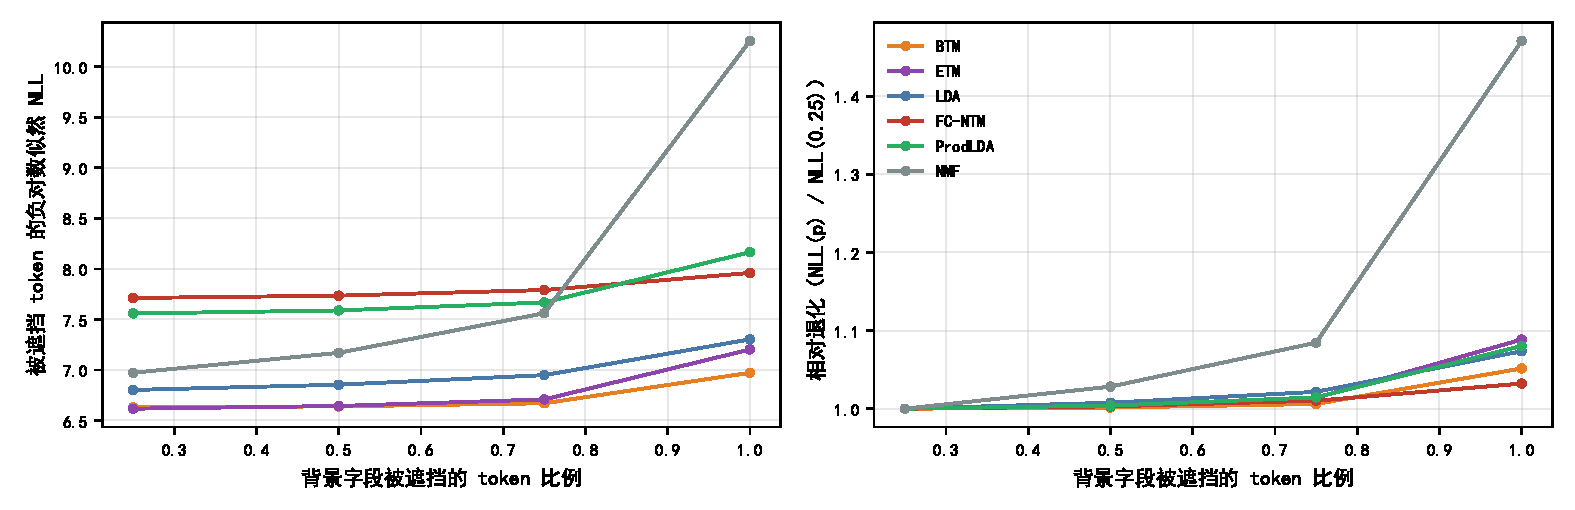
\includegraphics[width=0.86\textwidth]{fig_occlusion.pdf}
\caption{部分遮挡背景字段后的推断行为（GitHub issues，seed 11，测试集 2000 条）。
左：被遮挡 token 的每 token 负对数似然；右：相对退化
$\mathrm{NLL}(p)/\mathrm{NLL}(0.25)$，用于消除各模型词分布“锐利程度”不同带来的绝对尺度
差异。\fcntm{} 在训练时以 $p=0.5$ 随机整体置零背景字段，其相对退化最小（$\times$1.032），
说明在该基线集合下 \fcntm{} 对背景缺失的相对响应最小；这一比值本身不能区分“用概要补全”与“对输入不敏感”，机制归因仍需输入置换对照；但绝对 NLL 与主题一致率并非最优，
见表 \ref{tab:occl-robust}。}
\label{fig:occlusion}
\end{figure}

\begin{table}[t]
\centering
\caption{部分遮挡曲线对应的数值（GitHub issues，seed 11）。NLL 为被遮挡背景 token 的每
token 负对数似然（越低越好）；相对退化为 $\mathrm{NLL}(100\%)/\mathrm{NLL}(25\%)$；
一致率为遮挡 100\% 时与\emph{未遮挡}（$p=0$）时最可能主题相同的文档比例
（$p=0$ 行本身的一致率恒为 1，表中不列）。BTM 按其原文第 3.3 节的文档—主题推断
$p(z\mid d)$ 纳入本协议（见第 \ref{sec:fair-readout} 节）；
11/23/37 三个种子的跨语料汇总见表 \ref{tab:occl-cross}。}
\label{tab:occl-robust}
\small
\setlength{\tabcolsep}{4pt}
\begin{tabular}{@{}lccccc@{}}
\toprule
模型 & NLL(25\%) & NLL(50\%) & NLL(75\%) & NLL(100\%) & 相对退化 / 一致率(100\%) \\
\midrule
\fcntm{} & 7.712 & 7.735 & 7.790 & 7.960 & \textbf{1.032} / 0.358 \\
LDA & 6.802 & 6.854 & 6.948 & 7.302 & 1.074 / 0.420 \\
ProdLDA & 7.558 & 7.588 & 7.668 & 8.165 & 1.080 / 0.354 \\
BTM & 6.630 & 6.639 & 6.670 & \textbf{6.972} & 1.052 / 0.448 \\
ETM & \textbf{6.616} & 6.643 & 6.708 & 7.202 & 1.089 / 0.452 \\
NMF & 6.972 & 7.169 & 7.561 & 10.255 & 1.471 / \textbf{0.469} \\
\bottomrule
\end{tabular}
\end{table}

表 \ref{tab:occl-robust} 与图 \ref{fig:occlusion} 给出三点观察。第一，从遮挡 25\% 到
100\%，\fcntm{} 的每 token NLL 只上升 3.2\%（7.712$\rightarrow$7.960），而 LDA 上升 7.4\%、
ProdLDA 8.0\%、ETM 8.9\%、BTM 5.2\%、NMF 47.1\%；这与训练时以 0.5 的概率整体置零背景
字段一致。第二，绝对预测与主题稳定性并不由 \fcntm{} 领先：
完全遮挡时 BTM 的 NLL 最低（6.972）、ETM 次之，最可能主题一致率最高的是 NMF（0.469）与
ETM（0.452），\fcntm{} 为 0.358；因此本文只主张它的相对退化最小，不主张它在缺失字段下
预测最准。第三，三点限定同时成立：相对退化消除了不同词分布锐利程度的差异，而绝对 NLL 的
跨模型比较会混入校准差异；协议覆盖三个语料、各三个种子，掩码按种子重新抽样，但三个语料
都是英文、字段划分沿用题名/正文结构；“稳定”也可能来自对输入不敏感——本协议遮挡的正是
背景字段，稳定性本身不能证明模型用概要完成了补全，必须与绝对预测及读出匹配结果一起解读。

\subsection{跨语料对比：字段机制在什么条件下值得用}
\label{sec:cross-corpus}

同一协议在 AG News（$K=30$、测试集 7600 条）与土木工程文献
（$K=30$、测试集 2000 条）上运行，三个语料各取 11/23/37
三个随机种子，得到表 \ref{tab:occl-cross} 与图 \ref{fig:occl-cross}。

\begin{table}[t]
\centering
\caption{三个语料上的部分遮挡行为对比（11/23/37 三个种子，均值$\pm$标准差；遮挡掩码按种子
重新抽样）。相对退化为
$\mathrm{NLL}(100\%)/\mathrm{NLL}(25\%)$；一致率为完全遮挡时与\emph{未遮挡}推断时最可能
主题相同的比例，加粗单元格为该语料上相对退化最低的模型。“字段不对称度”用两个无需训练的
统计量刻画：背景/概要的平均词数比，以及背景词\emph{词型}中不出现在同一文档概要里的比例
（逐文档去重词型独有率，训练集统计；按出现次数加权的对应值见正文）。}
\label{tab:occl-cross}
\small
\setlength{\tabcolsep}{4pt}
\begin{tabular}{@{}llcc@{}}
\toprule
语料（字段不对称度） & 模型 & 相对退化 & 一致率(100\%) \\
\midrule
\multirow{6}{*}{\shortstack[l]{GitHub issues\\ 长度比 12.9\\ 背景独有 0.877}}
 & \fcntm{} & \textbf{1.029$\pm$0.003} & 0.345 \\
 & LDA & 1.074$\pm$0.000 & 0.424 \\
 & ProdLDA & 1.081$\pm$0.002 & 0.347 \\
 & ETM & 1.088$\pm$0.003 & 0.455 \\
 & BTM & 1.052$\pm$0.001 & 0.438 \\
 & NMF & 1.470$\pm$0.006 & 0.467 \\
\midrule
\multirow{6}{*}{\shortstack[l]{土木文献\\ 长度比 11.2\\ 背景独有 0.894}}
 & \fcntm{} & 1.010$\pm$0.001 & 0.673 \\
 & LDA & 1.036$\pm$0.002 & 0.561 \\
 & ProdLDA & 1.027$\pm$0.003 & 0.552 \\
 & ETM & 1.041$\pm$0.001 & 0.655 \\
 & BTM & \textbf{1.007$\pm$0.001} & 0.561 \\
 & NMF & 1.173$\pm$0.001 & 0.655 \\
\midrule
\multirow{6}{*}{\shortstack[l]{AG News\\ 长度比 3.9\\ 背景独有 0.868}}
 & \fcntm{} & 1.018$\pm$0.001 & 0.520 \\
 & LDA & \textbf{1.005$\pm$0.001} & 0.436 \\
 & ProdLDA & 1.026$\pm$0.001 & 0.489 \\
 & ETM & 1.072$\pm$0.001 & 0.554 \\
 & BTM & 1.044$\pm$0.001 & 0.555 \\
 & NMF & 1.408$\pm$0.003 & 0.546 \\
\bottomrule
\end{tabular}
\end{table}

\begin{figure}[t]
\centering
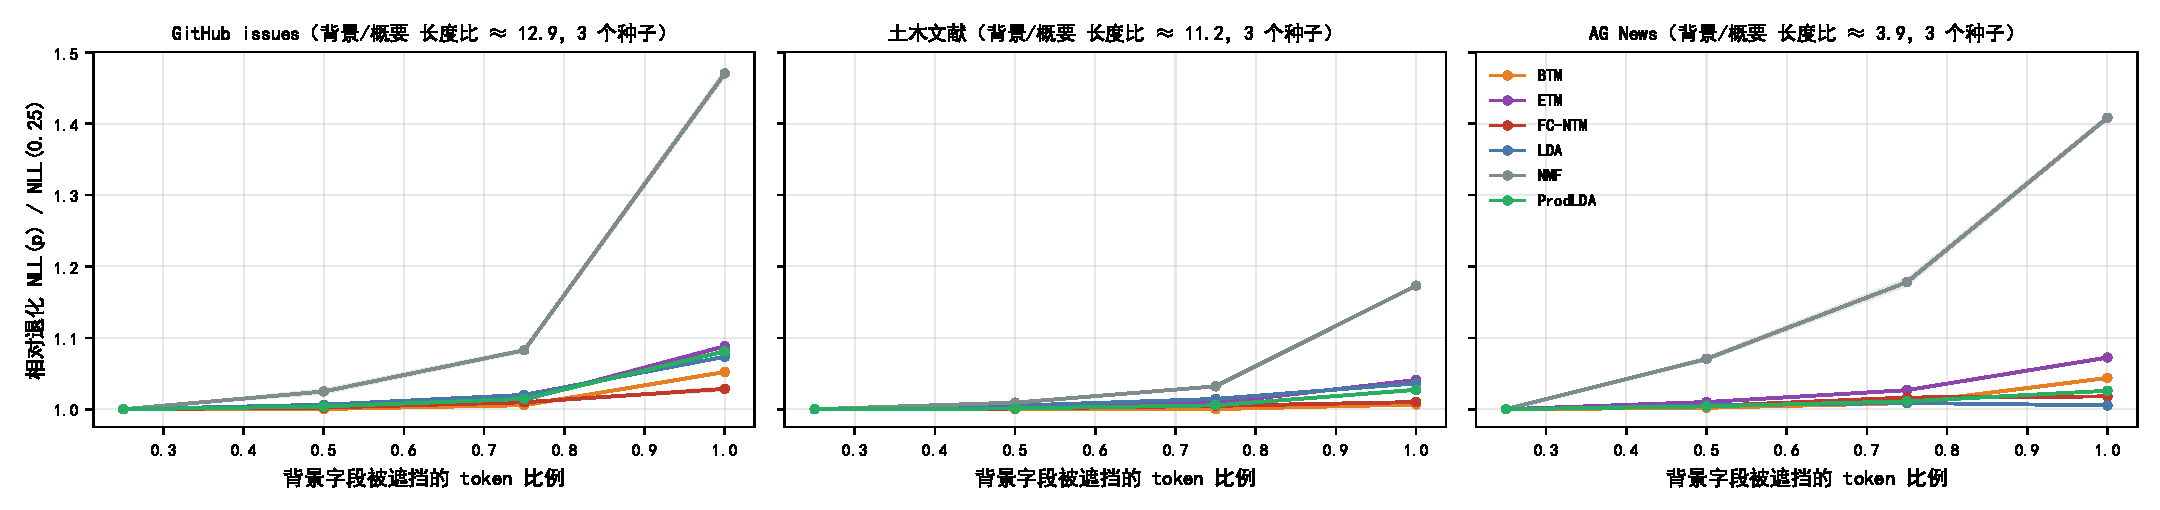
\includegraphics[width=0.86\textwidth]{fig_occlusion_cross_corpus.pdf}
\caption{同一部分遮挡协议在三个语料上的相对退化曲线（3 个种子，曲线为均值、阴影为
$\pm$1 标准差）。左：GitHub issues（背景/概要长度比 $\approx$12.9）；中：土木工程文献
（$\approx$11.2）；右：AG News（$\approx$3.9）。只有 GitHub 上 \fcntm{} 的退化明显小于
全部基线；土木文献与 AG News 上相对退化最小的分别是 BTM 与 LDA，\fcntm{} 与它们的差距
都在 0.003--0.013 以内。}
\label{fig:occl-cross}
\end{figure}

三点结论。第一，遮挡优势只在三个语料中的一个上测得，且与长度比不一致：GitHub（长度比
12.9）上所有模型都有可测退化（$\times$1.029--$\times$1.470），\fcntm{} 退化最小，按同
种子配对比最好基线 BTM 低 $+$0.024$\pm$0.004（3/3）；长度比几乎相同的土木文献（11.2）
上 \fcntm{}（1.010）不优于 BTM（1.007，配对差 $-$0.003$\pm$0.001，0/3 种子）；AG News
（3.9）上 \fcntm{}（1.018）也不优于 LDA（1.005，配对差 $-$0.013$\pm$0.000，0/3）。
第二，没有一个训练前统计量与三语料结果一致：按跨字段互预测，GitHub 反而更可预测
（$\rho^2_{\mathrm{cca}}$ 0.306 对 0.245）；长度比与背景独有内容占比只能区分 GitHub 与
AG News，无法区分 GitHub 与土木文献——后两者的统计量接近甚至更高，遮挡结论却相反；换成
token 加权口径（0.826 / 0.862 / 0.803）后仍无单调关系。第三，因此本文只把这两个统计量
作为语料描述，不把它们当前置判据；三个语料点在领域、文体与字段质量上同时变化，建立可用
的适用条件需要在更多语料上按固定协议标定并用独立语料检验。需要声明两点：AG News 与土木
文献上 \fcntm{} 与最好基线的差距只有 0.003--0.013，不宜据此宣称实际显著；NMF 为非概率
分解，在三个语料上退化都最大（$\times$1.47、$\times$1.41、$\times$1.17），说明该协议
对模型的词分布形式敏感。

\begin{figure}[t]
\centering
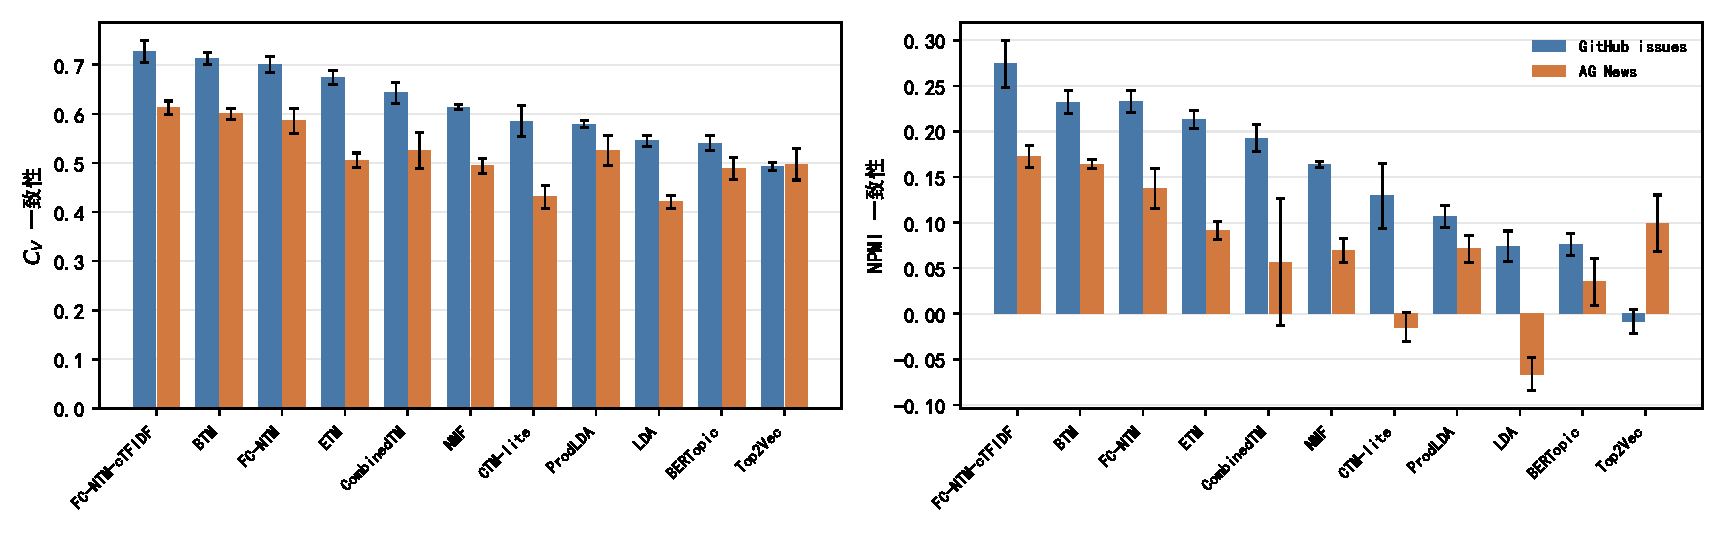
\includegraphics[width=0.86\textwidth]{fig_main_comparison.pdf}
\caption{两个公开语料上的主结果（统一评测词表、每主题 top-10 词）。左：$C_V$；右：NPMI。误差线为跨种子
标准差。GitHub 上 \fcntm{} 两行与 BTM、ETM，以及 AG News 的 \fcntm{} 两行均为 3 种子结果；
两个语料的 CombinedTM、ProdLDA 与 CTM-lite 也在同一协议下运行 11/23/37 三个种子。}
\label{fig:main}
\end{figure}

字段长度比阶梯与遮挡协议的机制对照见补充材料：两者都表明，长度比与相对退化只能作为描述量，不能作为机制收益的事前判据。

\subsection{字段视角评价}
\label{sec:fieldview}

\begin{table}[t]
\centering
\caption{\fcntm{} 的字段视角一致性（K=30，11/23/37 三个随机种子）。
该表是\emph{字段受限的主题词读出}：把同一个全局 $\beta$ 的行截断到某一字段的词表，再按该
字段的文档评测。它不是遮挡实验——$\beta$ 不随单篇文档的字段缺失改变。末列给出概要视角
真正参与平均的主题数：主题词局限于某一字段后，若该主题的前 10 个字段词在留出测试文本里
从不出现，gensim 的 $C_V$ 上下文向量为零向量、该主题的分数无定义，只能从均值中剔除
（三个语料的背景视角为 29--30/30）。}
\label{tab:fieldview}
\small
\begin{tabular}{lcccc r}
\toprule
语料 & 背景视角 $C_V$ & 背景视角 NPMI & 概要视角 $C_V$ & 概要视角 NPMI & 概要可评分主题 \\
\midrule
GitHub issues & 0.697$\pm$0.016 & 0.232$\pm$0.012 & 0.426$\pm$0.012 & $-$0.310$\pm$0.013 & 20--22 \\
AG News & 0.566$\pm$0.016 & 0.122$\pm$0.016 & 0.423$\pm$0.015 & $-$0.334$\pm$0.017 & 29--30 \\
土木文献 & 0.637$\pm$0.015 & 0.158$\pm$0.022 & 0.408$\pm$0.005 & $-$0.139$\pm$0.011 & 26--28 \\
\bottomrule
\end{tabular}
\end{table}

字段视角评价把主题词分别限定在两个字段的词表内，回答模型是否在两个字段上都组织出可读的
主题。表 \ref{tab:fieldview} 给出 \fcntm{} 的结果（与主表同一批模型）：三个语料上背景
视角的 $C_V$ 与全词表 $\beta$ 读出接近（0.697 / 0.566 / 0.637 对 0.701 / 0.586 / 0.633），
说明共享解码器在背景侧保留了大部分主题结构；概要视角的绝对值明显更低，主要来自评测口径
（概要只有 3--5 个词、参考语料极短），且 GitHub 上每个种子只有 20--22 个主题可评分
（AG News 29--30 个），该列是可评分主题子集上的均值，适合同口径比较而不宜与全词表数值直接
比大小。字段视角的跨模型对照见表 \ref{tab:fieldview-baselines}：把同一读出施加到 LDA、
BTM、NMF 与 ProdLDA 后，背景视角上 BTM 在 GitHub 与 AG News 略高于 \fcntm{}
（0.710 对 0.697、0.586 对 0.566），\fcntm{} 只在土木文献领先（0.637 对 NMF 0.600）；
概要视角上 LDA 与 ProdLDA 在三个语料上都高于 \fcntm{}（AG News 0.486 / 0.438 对 0.423）。
因此字段受限读出是任何具主题—词矩阵的模型都能计算的描述性读出，不能单独证明双编码器学到
了两个独立的字段主题结构；概要视角的负 NPMI 可以提出长度稀疏性假说，但在缺少长度匹配
对照的情况下不能断言它完全来自评测口径。
其中 \fcntm{} 自身的两个视角在 GitHub 上为 0.697$\pm$0.016 / 0.426$\pm$0.012
（NPMI 0.232$\pm$0.012 / $-$0.310$\pm$0.013）、在 AG News 上为 0.566$\pm$0.016 /
0.423$\pm$0.015（NPMI 0.122$\pm$0.016 / $-$0.334$\pm$0.017）、在土木文献上为
0.637$\pm$0.015 / 0.408$\pm$0.005（NPMI 0.158$\pm$0.022 / $-$0.139$\pm$0.011）；
概要视角的可评分主题数为 GitHub 20--22、AG News 29--30、土木文献 26--28（背景视角
29--30），该列是可评分主题子集上的均值。

\begin{table}[t]
\centering
\caption{字段受限读出的跨模型对照（$C_V$，11/23/37 三个种子的均值$\pm$标准差）。
每个模型的主题—词矩阵都按同一规则截断到字段词表，并只用该字段的测试文本评测；
“背景视角”为摘要/正文侧，“概要视角”为标题侧。}
\label{tab:fieldview}
\label{tab:fieldview-baselines}
\small
\setlength{\tabcolsep}{4pt}
\begin{tabular}{@{}llcc@{}}
\toprule
语料 & 模型 & 背景视角 $C_V$ & 概要视角 $C_V$ \\
\midrule
\multirow{5}{*}{GitHub issues}
 & \fcntm{} & 0.697$\pm$0.016 & 0.426$\pm$0.012 \\
 & BTM & \textbf{0.710$\pm$0.011} & 0.396$\pm$0.018 \\
 & NMF & 0.609$\pm$0.004 & 0.433$\pm$0.002 \\
 & LDA & 0.543$\pm$0.011 & 0.466$\pm$0.005 \\
 & ProdLDA & 0.575$\pm$0.006 & \textbf{0.467$\pm$0.034} \\
\midrule
\multirow{5}{*}{AG News}
 & \fcntm{} & 0.566$\pm$0.016 & 0.423$\pm$0.015 \\
 & BTM & \textbf{0.586$\pm$0.015} & 0.399$\pm$0.018 \\
 & NMF & 0.477$\pm$0.015 & 0.444$\pm$0.002 \\
 & LDA & 0.419$\pm$0.007 & \textbf{0.486$\pm$0.006} \\
 & ProdLDA & 0.499$\pm$0.032 & 0.438$\pm$0.007 \\
\midrule
\multirow{5}{*}{土木文献}
 & \fcntm{} & \textbf{0.637$\pm$0.015} & 0.408$\pm$0.005 \\
 & BTM & 0.589$\pm$0.014 & 0.382$\pm$0.008 \\
 & NMF & 0.600$\pm$0.009 & 0.398$\pm$0.013 \\
 & LDA & 0.554$\pm$0.008 & 0.415$\pm$0.006 \\
 & ProdLDA & 0.576$\pm$0.025 & \textbf{0.419$\pm$0.012} \\
\bottomrule
\end{tabular}
\end{table}

\subsection{消融：融合重构目标与门控}
\label{sec:fusion-ablation}

\begin{table}[t]
\centering
\caption{GitHub issues 上的三档融合消融（K=30，11/23/37 三个种子，统一协议，配对比较）。
同一读出内自上而下每次只改一处：先加上“把融合混合 $\theta_{\mathrm{fuse}}$ 本身解码进
重构项”（即式 \eqref{eq:lfuse}，均值融合），再把均值融合换成可学习门控（即主模型）。
“配对为正”为该行相对\emph{上一行}的逐种子配对差为正的种子数（$C_V$, NPMI）。另两个
对照（去掉融合重构项、以及用均值代替门控）的其余协议与主模型完全一致。}
\label{tab:fusion}
\small
\begin{tabular}{llcccc}
\toprule
读出 & 配置 & $C_V$ & NPMI & 配对为正 & UMass \\
\midrule
\multirow{3}{*}{$\beta$} & 不训练融合 & 0.721$\pm$0.016 & 0.266$\pm$0.012 & --- & $-$2.63 \\
 & 均值融合 $+$ 融合重构 & 0.708$\pm$0.016 & 0.245$\pm$0.013 & 1/3, 0/3 & $-$2.98 \\
 & 门控融合（主模型） & 0.701$\pm$0.016 & 0.233$\pm$0.012 & 0/3, 0/3 & $-$3.16 \\
\midrule
\multirow{3}{*}{cTFIDF} & 不训练融合 & 0.714$\pm$0.001 & 0.262$\pm$0.007 & --- & $-$1.86 \\
 & 均值融合 $+$ 融合重构 & 0.728$\pm$0.007 & 0.275$\pm$0.015 & 3/3, 3/3 & $-$1.91 \\
 & 门控融合（主模型） & 0.727$\pm$0.022 & 0.274$\pm$0.026 & 1/3, 1/3 & $-$1.90 \\
\bottomrule
\end{tabular}
\end{table}

表 \ref{tab:fusion} 用三档配置把两件事分开：是否为融合混合加一项重构目标，以及融合用均值
还是可学习门控。第一，\textbf{融合重构目标确实有效，但只对使用融合后验的读出有效}：在均值
融合下加上这一项后，cTFIDF 读出的 $C_V$ 与 NPMI 分别提高 0.014 与 0.013（3/3 种子为正），
而同一改动让 $\beta$ 读出下降 0.013 与 0.021。第二，\textbf{在本语料、本协议与三个种子下
没有观察到门控的额外收益}：把均值融合换成门控后，cTFIDF 读出的差值是 $-0.001$ 与 $-0.000$
（1/3 为正），$\beta$ 读出继续下降 0.007 与 0.012（0/3）。这一结论有明确边界：去掉融合
重构项时门控得不到梯度、参数精确退化为均值融合，因此该实验无法把“门控参数本身的价值”与
“融合目标的价值”分开，本文只报告未观察到额外收益，不主张已训练的门控普遍无用。该收益只
出现在 cTFIDF 上的原因是：融合重构项训练的正是 $\theta_{\mathrm{fuse}}$，而 cTFIDF 读出由
它聚合而来；$\beta$ 读出不经过它，因此这一项与两条流各自的重构目标竞争，略微牺牲了单流
主题词的质量。

\subsection{核心组件的消融}

\label{sec:core-ablation}

\begin{table}[t]
\centering
\caption{核心组件消融：三个语料、两种读出（$K=30$，11/23/37 三个种子，700 轮预算，其余协议
与主模型完全相同）。每一列相对\emph{同语料、同读出}的主模型只改一处：\emph{$-$跨字段重构}
关闭两条字段流各自的跨字段重构、\emph{$-$JS 一致性}把一致性权重设为 $0$、
\emph{$-$词掩码}关闭字段级词掩码、\emph{$-$字段置零}关闭背景字段整体置零；式
\eqref{eq:lfuse} 的融合重构项在四列中都保留。表内是逐种子配对差的均值 $\Delta C_V$
（负值表示去掉该组件后一致性下降），括号内为配对为正的种子数。主模型绝对值为
GitHub $\beta$ 0.701、类 TF-IDF 0.727；AG News $\beta$ 0.586、类 TF-IDF 0.612；
土木文献 $\beta$ 0.633、类 TF-IDF 0.636。前两个语料的字段长度比为 12.9 与 3.9，
土木文献为 11.2。}
\label{tab:core-ablation}
\small
\setlength{\tabcolsep}{5pt}
\begin{tabular}{llcccc}
\toprule
语料 & 读出 & $-$跨字段重构 & $-$JS 一致性 & $-$词掩码 & $-$字段置零 \\
\midrule
GitHub & $\beta$ & $+$0.021 (2/3) & $-$0.001 (1/3) & $-$0.012 (1/3) & $-$0.023 (1/3) \\
GitHub & 类 TF-IDF & $-$0.005 (1/3) & $+$0.004 (2/3) & $-$0.004 (1/3) & $-$0.021 (1/3) \\
\midrule
AG News & $\beta$ & $-$0.011 (2/3) & $+$0.003 (1/3) & $-$0.026 (0/3) & $-$0.010 (1/3) \\
AG News & 类 TF-IDF & $-$0.022 (0/3) & $-$0.002 (1/3) & $-$0.043 (0/3) & $-$0.023 (1/3) \\
\midrule
土木文献 & $\beta$ & $-$0.022 (0/3) & $+$0.001 (2/3) & $-$0.010 (1/3) & $+$0.001 (1/3) \\
土木文献 & 类 TF-IDF & $-$0.019 (0/3) & $-$0.002 (0/3) & $-$0.012 (0/3) & $-$0.034 (0/3) \\
\bottomrule
\end{tabular}
\end{table}

表 \ref{tab:core-ablation} 把四个组件在三个语料上逐一关闭，给出四点结论。第一，\textbf{JS
一致性项是唯一在三个语料、两种读出上都不承重的组件}（六格 $|\Delta C_V| \leq 0.004$）：
在本文参数化下，真正把融合表示训练起来的是融合重构目标，而不是把两条流后验拉近的正则。
第二，\textbf{跨字段重构与词掩码的承重情况随语料变化}：GitHub 上去掉跨字段重构后 $\beta$
读出反而高 0.021（2/3 为正）、类 TF-IDF 只低 0.005，去掉词掩码也只低 0.004；AG News 与
土木文献上去掉两者都使两种读出下降（跨字段重构 $-$0.011/$-$0.022 与 $-$0.022/$-$0.019，
词掩码 $-$0.026/$-$0.043 与 $-$0.010/$-$0.012，两个语料的类 TF-IDF 读出都是 0/3）。
第三，\textbf{字段整体置零的作用集中在类 TF-IDF 读出上，且并非在三个语料上都承重}：
GitHub 与 AG News 上两种读出都下降（$-$0.023、$-$0.021、$-$0.010、$-$0.023），土木文献上
$\beta$ 读出几乎不变（$+$0.001）、只有类 TF-IDF 读出下降 0.034。第四，\textbf{字段不
对称度不能解释组件层面的差异}：土木文献的长度比（11.2）与 GitHub（12.9）几乎相同，但组件
承重模式与 AG News（3.9）一致、与 GitHub 相反。三点范围说明：该消融关闭的是两条字段流各自
的跨字段重构，式 \eqref{eq:lfuse} 的融合重构项仍然让 $\theta^{\mathrm{fuse}}$ 同时重建两个
字段，因此“$-$跨字段重构”不等于完全切断字段间的信息流；AG News 与土木文献上多数差值只是
三个种子同向，按均值仍处于或接近种子波动量级；土木文献的字段文体与工程实践文档不同，其
结论不宜外推到其它文体。综合来看，本文只主张可复现的部分：类 TF-IDF 读出的增益来自融合
重构目标，JS 一致性项在三个语料上都不可分辨，跨字段重构与词掩码在 GitHub 上未观测到稳定
收益、在另两个语料上承重，字段整体置零的代价主要落在类 TF-IDF 读出上。

\subsection{融合重构权重的敏感性}

\label{sec:weight-sweep}

\begin{table}[t]
\centering
\caption{GitHub issues 上融合重构权重 $\lambda_f$ 的敏感性（门控融合，11/23/37 三个种子）。
$\lambda_f=0$ 即不训练融合（表 \ref{tab:fusion} 的第一档），$\lambda_f=0.5$ 是本文的取值；
其余协议与主模型完全一致。}
\label{tab:weight}
\small
\setlength{\tabcolsep}{4pt}
\begin{tabular}{lcccc}
\toprule
\multirow{2}{*}{$\lambda_f$} & \multicolumn{2}{c}{$\beta$ 读出} & \multicolumn{2}{c}{类 TF-IDF 读出} \\
 & $C_V$ & NPMI & $C_V$ & NPMI \\
\midrule
0 & 0.721$\pm$0.016 & 0.266$\pm$0.012 & 0.714$\pm$0.001 & 0.262$\pm$0.007 \\
0.25 & 0.697$\pm$0.015 & 0.217$\pm$0.031 & 0.713$\pm$0.015 & 0.262$\pm$0.004 \\
0.5 & 0.701$\pm$0.016 & 0.233$\pm$0.012 & 0.727$\pm$0.022 & 0.274$\pm$0.026 \\
1.0 & 0.716$\pm$0.012 & 0.246$\pm$0.026 & 0.723$\pm$0.012 & 0.277$\pm$0.018 \\
\bottomrule
\end{tabular}
\end{table}

表 \ref{tab:weight} 给出三点观察。$\lambda_f=0.25$ 明显过小：cTFIDF 读出几乎与不训练融合
相同（$C_V$ 0.713 对 0.714），而 $\beta$ 读出已下降 0.024；cTFIDF 的收益在 0.5 与 1.0 之间
几乎不变（$C_V$ 0.727 对 0.723、NPMI 0.274 对 0.277，差异都在 0.005 以内），说明它不是只在
0.5 出现的巧合；$\beta$ 读出的代价随权重增大而收窄（相对 $\lambda_f=0$ 从 $-0.020$ 缩到
$-0.005$）。因此 0.5 是“cTFIDF 收益”与“$\beta$ 代价”之间折中的保守取值。

\subsection{遮挡背景字段：真正的缺失推断实验}


\begin{table}[t]
\centering
\caption{把背景字段在\emph{推理期}整体置零后的缺失推断（K=30，最终配置，700 轮预算）。
$\Delta C_V$ 为同一读出协议下“完整字段推断”与“遮挡后重新推断”的主题一致性差；
$\Delta\mathrm{NLL}$ 为每 token 负对数似然增量；一致率为两次推断的最可能主题相同的文档
比例。同一语料内的两行使用同一批种子配对，用于隔离“背景字段整体置零”这一\emph{训练}设置
的作用：六个格子都是 11/23/37 三个种子的均值（置零列的 $C_V$/一致率标准差：GitHub
0.022/0.012、土木文献 0.014/0.018、AG News 0.014/0.003）。}
\label{tab:occlusion}
\small
\setlength{\tabcolsep}{4pt}
\begin{tabular}{llcccccc}
\toprule
语料 & 训练设置 & $C_V^{\mathrm{full}}$ & $C_V^{\mathrm{occ}}$ & $\Delta C_V$
 & $\Delta\mathrm{NLL}$（每 token） & 一致率 & 平均 JS \\
\midrule
GitHub & 置零（$p=0.5$） & 0.727 & 0.717 & $+$0.009 & $+$0.241 & 0.345 & 0.082 \\
       & 不置零 & 0.705 & 0.725 & $-$0.020 & $+$0.242 & 0.346 & 0.092 \\
\midrule
土木文献 & 置零（$p=0.5$） & 0.636 & 0.627 & $+$0.009 & $+$0.103 & 0.673 & 0.033 \\
        & 不置零 & 0.602 & 0.597 & $+$0.005 & $+$0.125 & 0.642 & 0.039 \\
\midrule
AG News & 置零（$p=0.5$） & 0.612 & 0.594 & $+$0.018 & $+$0.232 & 0.520 & 0.049 \\
        & 不置零 & 0.589 & 0.582 & $+$0.007 & $+$0.269 & 0.498 & 0.060 \\
\bottomrule
\end{tabular}
\end{table}

表 \ref{tab:occlusion} 给出真正的遮挡推断结果。第一，把背景字段整体置零后，主题词一致性
\emph{几乎不变}（六个格子的 $\Delta C_V$ 都在 $\pm$0.02 以内，GitHub 三个种子上的符号还会
翻转）：主题词一致性对字段缺失不敏感，若同时改变主题词候选词表与参考语料，度量到的会是
评测口径而不是信息损失。第二，信息损失真实存在，但出现在文档级后验与词级预测上：遮挡后
约 66\%（GitHub）与 48\%（AG News）的文档改变了最可能主题，每 token 负对数似然上升
0.24/0.23（置零训练）或 0.24/0.27（不置零）；因此“背景字段携带独立信息”应当用
$\Delta\mathrm{NLL}$、主题一致率或缺失补全指标论证。第三，该结果不足以说明字段整体置零
带来预测性能收益：三种子均值下，启用置零的模型在完整输入与遮挡后的绝对 NLL 都更高，它改变
的是\emph{增量}与后验稳定性，且这一效果依语料——AG News 上置零把每 token 增量从 0.269
降到 0.232、一致率从 0.498 提到 0.520、JS 从 0.060 降到 0.049；土木文献同向
（0.125$\rightarrow$0.103、JS 0.039$\rightarrow$0.033）；GitHub 上增量几乎相同（0.242 对
0.241），只有 JS 略低（0.092$\rightarrow$0.082）。也就是说，置零训练在两个语料上减小了
字段缺失带来的后验漂移，在 GitHub 上不出现，也不能替代绝对预测精度；要确认这一点仍需
“仅见标题”的对照模型与文档层面的不确定性，这些尚未完成。把置零与不置零配对起来看，三个
语料一致的部分是：置零训练的完整输入 $C_V$ 更高（GitHub 0.727 对 0.705、AG News 0.612 对
0.589、土木文献 0.636 对 0.602），但其绝对 NLL 也更高，说明它改变的是主题词一致性与后验
分布的形状，而不是词级预测的校准。

\subsection{冗余度度量与增益的关系}



补充材料的冗余度表给出留出冗余度度量（训练集拟合、测试集评估）。两个语料的留出
互预测能力接近，GitHub 略高（$\rho^2_{\mathrm{cca}}$ 0.306 对 0.245），而
\fcntm{}-cTFIDF 在 3 种子子集上于两个语料都略高于 BTM（读出匹配下 $+$0.027 与 $+$0.019）；
10 种子配对显示只有 GitHub 的优势保持（$+$0.028，9/10），AG News 变为 $-$0.009（3/10）。
也就是说，现有证据既不支持“互补才有增益”，也不支持“冗余就有代价”；两种口径下的 $C_V$
差距（0.019--0.027 与 0.012--0.014）与种子间波动处于同一量级，因此只能说“略高于最强经典
基线”，不能写成显著优于。遮挡诊断与冗余度的方向同样不一致：真实遮挡下两个语料的
$\Delta C_V$ 都接近 0（GitHub $+$0.009$\pm$0.022、AG News $+$0.018$\pm$0.013），幅度与
种子间波动同量级。因此本文不采用“跨字段冗余度可以事先预测增益”的说法；要建立这样的判据，
需要在更多语料上按固定协议标定并用独立语料检验预测能力。


\subsection{主题样例}


补充材料给出主题样例（自动生成）。
需要说明：在 GitHub 语料上，两个字段的词表高度重叠（概要词表 3458 词几乎全部出现在
背景词表中），因此分字段截断后多数主题两侧给出同一批词，样例并不能单独支撑“两个字段学会了不同分工”的结论。这也说明主题样例必须从训练模型
的输出直接生成：手工挑选的词可能被语料特有的停用词表过滤、或根本不在 5175 词的
评测词表内。

\section{讨论与局限}

本文认为，双字段短文本主题建模的价值需要分开陈述：可以复现的是\textbf{表示层}的能力——
同一训练结果能给出字段受限的主题词读出，并且在背景字段缺失时仍能推断出主题比例
（GitHub 上遮挡后最可能主题改变者占 66\%、每 token 负对数似然上升 0.24，3 个种子）；
而\textbf{通用一致性
指标}上的优势依语料：在\emph{读出匹配}的条件下，10 种子配对只在 GitHub 上观测到
\fcntm{}-cTFIDF 高于最强经典基线 BTM $+$0.028（95\% CI 不含 0，9/10），AG News 上为
$-$0.009（CI 含 0，3/10）。

这与“互补语料受益、冗余语料受损”的简单假设不同，原因有两层。其一，主题质量指标对实现
细节（解码方式、训练预算与蒙特卡洛噪声）敏感，因此在统一协议下实测比沿用直觉更可靠；
其二，留出冗余度度量本身显示 GitHub 反而略更可预测（更“冗余”）。因此本文不把冗余度当作
增益方向的解释变量，只把它作为描述语料字段关系的两个指标报告。

对工程文献管理而言，该协议可以直接落在标题—摘要语料上：字段受限的主题词读出更贴近“标题词与摘要词”的实际用法，遮挡推断对应摘要缺失时的主题估计；因此即使通用一致性指标上
的增益有限，字段级读出与缺失推断仍具有工程使用价值。

本文存在以下局限。第一，三个语料都是英文，字段划分依赖既有的标题/正文结构，对字段边界需要
自动识别的场景尚未验证；GitHub 的背景字段还有极长的长尾（最长 20532 个 token），依赖句向量
的基线按 128 token 截断，补充材料给出窗口池化的控制。第二，留出冗余度量只在
两个语料上计算，二者互预测能力接近（$\rho^2_{\mathrm{cca}}$ 0.306 对 0.245），而 10 种子
配对只在 GitHub 上观测到正增益，因此既没有“冗余度决定增益”的单调关系，也无法给出“冗余度
高于多少就不值得建模字段结构”的阈值；建立前置判据需要在更多语料上标定并用独立语料检验。
第三，非参数基线（BERTopic、Top2Vec）的主题数不由 $K$ 决定（Top2Vec 在 AG News 上退化为
2--4 个主题），其数值只作参考。第四，字段视角读出对任何具主题—词矩阵的模型都可计算，对照
显示它不是双编码器独有的优势（背景视角 BTM 在 GitHub 与 AG News 略高，概要视角 LDA/ProdLDA
更高），因此本文只把它作为描述性读出。第五，词掩码率、整体置零概率与融合重构权重均取经验
值，其与语料规模、字段长度比的交互尚未系统刻画；所有神经模型都用 20\% 训练文档做早停验证，
而 \fcntm{} 的类 TF-IDF 读出用全部训练文档的后验聚合，“优化用样本数”与“读出用样本数”
不同，不能笼统写成只对 \fcntm{} 不利。第六，全部数字来自同一套协议（$K=30$、700 轮预算、
统一读出与评测词表）；\fcntm{} 与 BTM 在两个语料上各扩展到 10 个种子，其余基线与土木文献
仍为 3 种子，因此多种子推断的读出对比覆盖 \fcntm{} 与 BTM，遮挡对比另覆盖 LDA（AG News）；
类 TF-IDF 读出是唯一优势口径——在 $\beta$ 读出下 \fcntm{} 在两个语料上都低于 BTM 的原生
$\beta$ 读出（$-$0.014 与 $-$0.027）。第七，遮挡实验的覆盖范围需要分开陈述：整字段遮挡在
三个语料上都有两种训练设置、各 11/23/37 三个种子；部分遮挡的入口固定使用置零训练的检查点，
置零与不置零两套曲线都已补齐（见补充材料），但新增的 7 个种子只扩展了
置零设置，因此字段视角与部分遮挡曲线的多种子配对仍只覆盖该设置。最后，本文没有加入同预算、
同读出的单编码器或简单拼接对照，因此“双流协同结构本身是否更优”仍未被隔离，独立确认语料
也留作后续工作。

\section{结论}

本文面向双字段短文本提出字段协同神经主题模型 \fcntm：为两个字段分别建立条件变分流，以
跨字段重构与一致性正则把字段关系编码进共享主题空间，以字段级词掩码与背景字段整体置零处理
部分观测与整体缺失，并把文档级融合表示真正纳入训练目标。在读出层面，本文对所有模型采用
同一词表与同一主题词数量的统一协议，消除了跨模型比较中由词表范围与主题词长度差异造成的
偏差。

在 GitHub issues 与 AG News 两个公开语料上，\fcntm{} 的结果依语料：在读出匹配的条件下
（BTM 也按原文第 3.3 节导出文档—主题后验并使用同一类 TF-IDF 读出），10 种子配对显示
类 TF-IDF 读出在 GitHub 上比最强的经典基线 BTM 高 $+$0.028 $C_V$
（95\% CI [$+$0.012, $+$0.043]，9/10；主表 3 种子均值 0.727 对 0.700、NPMI 0.274 对
0.235），在 AG News 上为 $-$0.009（CI 含 0，3/10；0.612 对 0.593）。我们同时给出并实测了
两个字段关系度量：留出双向互预测
（含留出平方典型相关）与\emph{训练后}的遮挡推断诊断。这些结论是保守的，也是可检验的：
两个语料的字段冗余度接近，但增益并不在两个语料上同时出现，因此本文的数据不支持
“冗余度决定增益”这一前置判据；把背景字段在推理期整体置零后主题词一致性几乎不变，
真正的信息损失体现在文档级后验与词级预测上。本文的主张是：\fcntm{} 提供了可复现的
字段视角读出、缺失字段推断行为，以及在读出匹配的条件下、在 GitHub 上得到 10 种子支持的
小幅提升（$+$0.028 $C_V$，95\% CI 不含 0；AG News 上未观测到优势）。是否值得为字段
结构付出额外的建模代价，应当按本文协议在目标语料上实测，而不是由冗余度预先判定。
在部分遮挡协议下，\fcntm{} 只在 GitHub 上表现出最小的相对退化
（$\times$1.029$\pm$0.003；按种子配对，3/3 个种子都优于同一种子上最好的基线 BTM，
配对差 $+$0.024$\pm$0.004；扩到 10 种子后优势保持：$+$0.024，10/10，$p=0.002$），
这是该协议与基线集合下的诊断证据（它衡量的是相对退化，不是主题词的通用一致性；
打乱概要的对照见补充材料；组件消融见第 \ref{sec:core-ablation} 节）；
在土木文献（长度比 11.2）与 AG News 上它都不占优（相比各自同种子最好的基线 BTM 与 LDA，
配对差 $-$0.003$\pm$0.001 与 $-$0.013$\pm$0.000，都是 0/3 种子；AG News 扩到 10 种子后
仍为 $-$0.013、0/10），并且它的主题一致率在 GitHub 与 AG News 上不是最高（在土木文献上最高），说明
“鲁棒”与“更准”是两个需要分开报告的性质。
遮挡优势与训练前统计量的关系因此是否定的：长度比与背景独有内容占比（逐文档去重词型独有率；
token 加权口径分别为 0.826、0.862、0.803）能区分 GitHub（12.9 / 0.877，占优）与 AG News
（3.9 / 0.868，不占优），但无法区分 GitHub 与统计量几乎相同、背景独有内容甚至更高的土木
文献（11.2 / 0.894，不占优）；固定文献与词表、只改变摘要长度的
阶梯实验也没有给出与长度比一致的组件承重模式（$\beta$ 读出的跨字段重构在 abs60 档甚至
3/3 种子为正）。因此本文不把这两个统计量当作事前判据，只把它们作为语料描述，并把建立
适用条件的任务留给后续工作（见第 \ref{sec:cross-corpus} 节与补充材料）。第三个语料（土木文献）的组件消融同样
显示，其承重模式与 AG News 一致而与 GitHub 相反，说明长度比也不能解释组件层面的差异——
这一否定结果写在第 \ref{sec:core-ablation} 与第 \ref{sec:cross-corpus} 节。

\section*{补充材料}
本文的附加实验与对照随论文以补充材料（Supplementary Material）单独提供，包含：
长文档截断的公平性控制、字段长度比阶梯、遮挡协议的机制对照、$\beta$ 读出敏感性、
字段冗余度度量表与图，以及主题样例表；正文中相应的引用均指向该补充材料。

\begin{thebibliography}{99}
\small
\bibitem{blei2003lda} Blei D M, Ng A Y, Jordan M I. Latent Dirichlet allocation[J]. Journal of Machine Learning Research, 2003, 3: 993--1022.
\bibitem{yin2014gsdmm} Yin J, Wang J. A Dirichlet multinomial mixture model-based approach for short text clustering[C]//Proceedings of the 20th ACM SIGKDD, 2014: 233--242.
\bibitem{srivastava2017avitm} Srivastava A, Sutton C. Autoencoding variational inference for topic models[C]//International Conference on Learning Representations, 2017.
\bibitem{miao2016nvdm} Miao Y, Yu L, Blunsom P. Neural variational inference for text processing[C]//Proceedings of ICML, 2016: 1727--1736.
\bibitem{bianchi2021ctm} Bianchi F, Terragni S, Hovy D. Pre-training is a hot topic: Contextualized document embeddings improve topic coherence[C]//Proceedings of ACL-IJCNLP (Volume 2: Short Papers), 2021: 759--766. DOI: 10.18653/v1/2021.acl-short.96.
\bibitem{dieng2020etm} Dieng A B, Ruiz F J R, Blei D M. Topic modeling in embedding spaces[J]. Transactions of the Association for Computational Linguistics, 2020, 8: 439--453.
\bibitem{wu2024survey} Wu X, Nguyen T, Luu A T. A survey on neural topic models: Methods, applications, and challenges[J]. Artificial Intelligence Review, 2024, 57: article 18. DOI: 10.1007/s10462-023-10661-7.
\bibitem{kurle2019multisource} Kurle R, G\"unnemann S, van der Smagt P. Multi-source neural variational inference[C]//Proceedings of AAAI, 2019: 4114--4121. DOI: 10.1609/aaai.v33i01.33014114.
\bibitem{zhang2017robust} Zhang G, Iwata T, Kashima H. Robust multi-view topic modeling by incorporating detecting anomalies[C]//ECML PKDD, LNCS 10535, 2017: 238--250. DOI: 10.1007/978-3-319-71246-8\_15.
\bibitem{pergola2021disentangled} Pergola G, Gui L, He Y. A disentangled adversarial neural topic model for separating opinions from plots in user reviews[C]//Proceedings of NAACL-HLT, 2021: 2870--2883. DOI: 10.18653/v1/2021.naacl-main.228.
\bibitem{liu2022dualview} Liu W, Huang Y, Guo Y, et al. Topic modeling for short texts via dual view collaborate optimization[C]//2022 7th IEEE International Conference on Data Science in Cyberspace (DSC), 2022: 160--166. DOI: 10.1109/DSC55868.2022.00028.
\bibitem{esmaeili2019structured} Esmaeili B, Huang H, Wallace B C, van de Meent J W. Structured neural topic models for reviews[C]//Proceedings of AISTATS (PMLR 89), 2019: 3429--3439.
\bibitem{card2018metadata} Card D, Tan C, Smith N A. Neural models for documents with metadata[C]//Proceedings of the 56th Annual Meeting of the Association for Computational Linguistics (Volume 1: Long Papers), 2018: 2031--2040. DOI: 10.18653/v1/P18-1189.
\bibitem{suzuki2017jmvae} Suzuki M, Nakayama K, Matsuo Y. Joint multimodal learning with deep generative models[EB/OL]. arXiv:1611.01891, 2016（首次提交于 2016-11，另有 ICLR 2017 投稿记录）.
\bibitem{nguyen2026subntm} Nguyen T, Doan D T, Luong H T, et al. Sub-document neural topic model[J]. Knowledge-Based Systems, 2026, 331: 114762. DOI: 10.1016/j.knosys.2025.114762.
\bibitem{zhu2018graphbtm} Zhu Q, Feng Z, Li X. GraphBTM: Graph enhanced autoencoded variational inference for biterm topic model[C]//Proceedings of EMNLP, 2018: 4663--4672. DOI: 10.18653/v1/D18-1495.
\bibitem{zhang2020bcktm} Zhang K, Zhou Y, Chen Z, et al. Incorporating biterm correlation knowledge into topic modeling for short texts[J]. The Computer Journal, 2022, 65(3): 537--553. DOI: 10.1093/comjnl/bxaa079.
\bibitem{vorontsov2015bigartm} Vorontsov K, Frei O, Apishev M, et al. BigARTM: Open source library for regularized multimodal topic modeling of large collections[C]//Analysis of Images, Social Networks and Texts (AIST 2015), CCIS 542, 2015: 370--381. DOI: 10.1007/978-3-319-26123-2\_36.（正则项的具体形式见官方文档 \url{https://docs.bigartm.org}，本文未复现）
\bibitem{roberts2019stm} Roberts M E, Stewart B M, Tingley D. stm: An R package for structural topic models[J]. Journal of Statistical Software, 2019, 91(2): 1--40.
\bibitem{zhang2015char} Zhang X, Zhao J, LeCun Y. Character-level convolutional networks for text classification[C]//Advances in Neural Information Processing Systems, 2015: 649--657.
\bibitem{openindex2026} open-index. Open GitHub issues: GitHub issue records by repository[DS/OL]. Hugging Face, 2026（快照日期 2026-06）. \url{https://huggingface.co/datasets/open-index/open-github-issues}.
\bibitem{openalex2022} Priem J, Piwowar H, Orr R. OpenAlex: A fully-open index of scholarly works, authors, venues, institutions, and concepts[EB/OL]. arXiv:2205.01833, 2022. \url{https://openalex.org}.
\bibitem{roder2015coherence} R\"oder M, Both A, Hinneburg A. Exploring the space of topic coherence measures[C]//Proceedings of WSDM, 2015: 399--408.
\bibitem{bouma2009npmi} Bouma G. Normalized (pointwise) mutual information in collocation extraction[C]//Proceedings of the Biennial GSCL Conference, 2009: 31--40.
\bibitem{lau2014tea} Lau J H, Newman D, Baldwin T. Machine reading tea leaves: Automatically evaluating topic coherence and topic model quality[C]//Proceedings of EACL, 2014: 530--539.
\bibitem{webber2010rbo} Webber W, Moffat A, Zobel J. A similarity measure for indefinite rankings[J]. ACM Transactions on Information Systems, 2010, 28(4): article 20, 1--38.
\bibitem{bischof2012exclusivity} Bischof J, Airoldi E M. Summarizing topical content with word frequency and exclusivity[C]//Proceedings of ICML, 2012: 201--208.
\bibitem{yan2013btm} Yan X, Guo J, Lan Y, et al. A biterm topic model for short texts[C]//Proceedings of the 22nd International World Wide Web Conference, 2013: 1445--1456.
\bibitem{lee2001nmf} Lee D D, Seung H S. Algorithms for non-negative matrix factorization[C]//Advances in Neural Information Processing Systems, 2001: 556--562.
\bibitem{grootendorst2022bertopic} Grootendorst M. BERTopic: Neural topic modeling with a class-based TF-IDF procedure[J/OL]. arXiv:2203.05794, 2022.
\bibitem{angelov2020top2vec} Angelov D. Top2Vec: Distributed representations of topics[J/OL]. arXiv:2008.09470, 2020.
\bibitem{reimers2019sbert} Reimers N, Gurevych I. Sentence-BERT: Sentence embeddings using Siamese BERT-networks[C]//Proceedings of EMNLP-IJCNLP, 2019: 3982--3992.
\bibitem{srivastava2014dropout} Srivastava N, Hinton G, Krizhevsky A, et al. Dropout: A simple way to prevent neural networks from overfitting[J]. Journal of Machine Learning Research, 2014, 15: 1929--1958.
\bibitem{prechelt1998early} Prechelt L. Early stopping---but when?[M]//Neural Networks: Tricks of the Trade. Berlin: Springer, 1998: 55--69.
\bibitem{dvbtm2022} Wei Liu, Yutao Huang, Yibing Guo, et al. Topic Modeling for Short Texts Via Dual View Collaborate optimization[C]//IEEE International Conference on Data Science in Cyberspace. 2022: 3, 160-166. DOI:10.1109/dsc55868.2022.00028.
\bibitem{crntm2020} Jiachun Feng, Zusheng Zhang, Cheng Hua Ding, et al. Context reinforced neural topic modeling over short texts[J]//Information Sciences. 2022: 607, 79-91. DOI:10.1016/j.ins.2022.05.098.
\bibitem{dvidtm2026} Di Liu, Zheng Fang, Bin Wu. DVI-DTM: Dual-View Representation Learning for Interpretable Short Text Dynamic Topic Modeling[C]//Annual Meeting of the Association for Computational Linguistics (ACL). 2026: 28576-28593. DOI:10.18653/v1/2026.acl-long.1318.
\bibitem{quantization2020} Xiaobao Wu, Chunping Li, Yan Zhu, et al. Short Text Topic Modeling with Topic Distribution Quantization and Negative Sampling Decoder[C]//Conference on Empirical Methods in Natural Language Processing (EMNLP). 2020: 1772-1782. DOI:10.18653/v1/2020.emnlp-main.138.
\bibitem{relationalbtm2018} Ximing Li, Ang Zhang, Changchun Li, et al. Relational Biterm Topic Model: Short-Text Topic Modeling using Word Embeddings[J]//The Computer Journal. 2018: 62(3), 359-372. DOI:10.1093/comjnl/bxy037.
\bibitem{sparsebtm2021} Bingshan Zhu, Yi Cai, Huakui Zhang. Sparse Biterm Topic Model for Short Texts[J]//Lecture notes in computer science. 2021: 227-241. DOI:10.1007/978-3-030-85896-4\_19.
\bibitem{civilnlp2023} Alireza Shamshiri, Kyeong Rok Ryu, June Young Park. Text mining and natural language processing in construction[C]//Automation in Construction. 2023: 158, 105200-105200. DOI:10.1016/j.autcon.2023.105200.
\bibitem{civilnlp2021} Chengke Wu, Xiao Li, Yuanjun Guo, et al. Natural language processing for smart construction: Current status and future directions[C]//Automation in Construction. 2021: 134, 104059-104059. DOI:10.1016/j.autcon.2021.104059.
\bibitem{civilaccident2018} Fan Zhang, Hasan A. Fleyeh, Xinru Wang, et al. Construction site accident analysis using text mining and natural language processing techniques[C]//Automation in Construction. 2018: 99, 238-248. DOI:10.1016/j.autcon.2018.12.016.
\bibitem{civilsafety2015} Antoine J.‐P. Tixier, Matthew Ryan Hallowell, Balaji Rajagopalan, et al. Automated content analysis for construction safety: A natural language processing system to extract precursors and outcomes from unstructured injury reports[C]//Automation in Construction. 2015: 62, 45-56. DOI:10.1016/j.autcon.2015.11.001.
\bibitem{civiltopic2024} Peng Chao Zhou, Yifan Qi, Qian Yang, et al. Neural topic modeling of machine learning applications in building: Key topics, algorithms, and evolution patterns[C]//Automation in Construction. 2024: 170, 105890-105890. DOI:10.1016/j.autcon.2024.105890.
\bibitem{duet2019} Yan Wang, John Eric Taylor. DUET: Data-Driven Approach Based on Latent Dirichlet Allocation Topic Modeling[C]//Journal of Computing in Civil Engineering. 2019: 33(3). DOI:10.1061/(asce)cp.1943-5487.0000819.
\bibitem{risknlp2023} Hieu T. T. L. Pham, SangUk Han. Natural Language Processing with Multitask Classification for Semantic Prediction of Risk-Handling Actions in Construction Contracts[C]//Journal of Computing in Civil Engineering. 2023: 37(6). DOI:10.1061/jccee5.cpeng-5218.
\bibitem{compliance2013} D. M. Salama, Nora El-Gohary. Semantic Text Classification for Supporting Automated Compliance Checking in Construction[C]//Journal of Computing in Civil Engineering. 2013: 30(1). DOI:10.1061/(asce)cp.1943-5487.0000301.
\bibitem{ontology2015} Peng Zhou, Nora El-Gohary. Ontology-Based Multilabel Text Classification of Construction Regulatory Documents[C]//Journal of Computing in Civil Engineering. 2015: 30(4). DOI:10.1061/(asce)cp.1943-5487.0000530.
\bibitem{contract2022} Seonghyeon Moon, Seokho Chi, Seok-Been Im. Automated detection of contractual risk clauses from construction specifications using bidirectional encoder representations from transformers (BERT)[C]//Automation in Construction. 2022: 142, 104465-104465. DOI:10.1016/j.autcon.2022.104465.
\end{thebibliography}

\end{document}
